\documentclass[11pt]{article}
\usepackage[letterpaper,margin=0.5in,nohead,nofoot]{geometry}
\usepackage{color}
\usepackage{amsfonts}
\usepackage{amssymb}
\usepackage{amsmath}
\usepackage{setspace}
\usepackage{graphicx}

%change2

\everymath{\displaystyle}
\onehalfspacing

%\newcommand{\bra}[1]{\langle #1|}
%\newcommand{\ket}[1]{|#1\rangle}
\newcommand{\braket}[2]{\langle #1|#2\rangle}
\mathchardef\minus = "002D

\newcommand{\swY}[4][]{{}_{{}_{#2}}\!Y^{#1}_{#3}(#4)}
\newcommand{\swSH}[5][]{{}_{{}_{#2}}S^{#1}_{#3}(#4;#5)}
\newcommand{\swS}[5][]{{}_{{}_{#2}}S^{#1}_{#3}(#4;#5)}
\newcommand{\scA}[4][]{{}_{{}_{#2}}A^{#1}_{#3}(#4)}
\newcommand{\YSH}[3][]{\mathcal{A}^{#1}_{#2}(#3)}

\makeatletter
\def\lambdabar{\protect\@lambdabar}
\def\@lambdabar{%
\relax
\bgroup
\def\@tempa{\hbox{\raise.73\ht0
\hbox to0pt{\kern.25\wd0\vrule width.5\wd0
height.1pt depth.1pt\hss}\box0}}%
\mathchoice{\setbox0\hbox{$\displaystyle\lambda$}\@tempa}%
{\setbox0\hbox{$\textstyle\lambda$}\@tempa}%
{\setbox0\hbox{$\scriptstyle\lambda$}\@tempa}%
{\setbox0\hbox{$\scriptscriptstyle\lambda$}\@tempa}%
\egroup
}
\makeatother

\begin{document}
\noindent{\large\bf Quasi-normal Mode Decomposition for the ring-down} \\

\noindent
Teukolsky general field solution:
\begin{equation}
\psi(t,r,\theta,\phi) = \frac{1}{2\pi} \int {e^{-i\omega t} \sum_{\ell,m} \swSH{s}{\ell{m}}{\theta,\phi}{a\omega}R_{\ell{m}}(r) d\omega },
\end{equation}
where the summation over $\ell$ and $m$ is always confined to $|s|<
\ell < \infty$ and $|m| \leq \ell$. To represent outgoing
gravitational waves, we use $s=-2$ and $\psi = \rho^{-4}\Psi_4$, with
$\Psi_4$ being the Weyl scalar that behaves like an 
outgoing gravitational wave at large distances and $\rho\equiv-1/(r-ia\cos\theta)$.
Asymptotically, $R_{lm}(r)=r^3e^{i\omega r^*}$ ($r^*$ is the
``tortoise'' radial coordinate), $\rho=1/r$, and we find
\begin{equation}
\Psi_4 \sim \frac1{r}\frac{1}{2\pi} \int {e^{-i\omega (t-r^*)} \sum_{\ell,m} \swSH{\minus 2}{\ell{m}}{\theta,\phi}{a\omega} d\omega }.
\end{equation}
Making both sides dimensionless, we take as our general asymptotic expansion for outgoing gravitational waves:
\begin{equation}
rM\Psi_4 = \frac{M}{2\pi} \int {e^{-i\omega (t-r^*)} \sum_{\ell,m} \swSH{\minus 2}{\ell{m}}{\theta,\phi}{a\omega} d\omega }.
\end{equation}

To represent the ring-down of a Kerr black hole, we replace the
Fourier integral with a QNM expansion (a careful assumption, because
QNMs are not a complete set).  For each mode $(\ell,m)$, there are
two infinite sets of QNMs labeled by $n$: $\bar\omega_{\ell{m}n}$ and
$\bar\omega^\prime_{\ell{m}n}$.  The $n=0$ modes represent the
dominant QNM for each $(\ell,m)$, and the higher values of $n$
represent overtones.  When we replace the integral with a sum over all QNM, we must include both sets of modes:
\begin{equation}
rM\Psi_4 = \sum_{\ell{m}n}\left\{C_{\ell{m}n}e^{-i\bar\omega_{\ell{m}n} (t-r^*)}
           \swSH{\minus 2}{\ell{m}}{\theta,\phi}{a\bar\omega_{\ell{m}n}} 
           + C^\prime_{\ell{m}n}e^{-i\bar\omega^\prime_{\ell{m}n} (t-r^*)}
           \swSH{\minus 2}{\ell{m}}{\theta,\phi}{a\bar\omega^\prime_{\ell{m}n}}
           \right\}, 
\end{equation}
where $C_{\ell{m}n}$ and $C^\prime_{\ell{m}n}$ are the arbitrary
dimensionless complex coefficients of the QNM expansion.

The two sets of QNMs for Kerr are closely related to each other.  The $\bar\omega$ correspond to ``positive frequency'' modes and the $\bar\omega^\prime$ to ``negative frequency'' modes in the following sense.  Let us define:
\begin{align}
    \bar\omega_{\ell{m}n} &\equiv 
    \omega_{\ell{m}n} - \frac{i}{\tau_{\ell{m}n}}
      &;\quad a\bar\omega_{\ell{m}n}\equiv c_{\ell{m}n}
    &\quad:\quad\mbox{and}\quad \omega_{\ell{m}n} \ge 0, \\
    \bar\omega^\prime_{\ell{m}n} &\equiv 
    \omega^\prime_{\ell{m}n} - \frac{i}{\tau^\prime_{\ell{m}n}}
      &;\quad a\bar\omega^\prime_{\ell{m}n}\equiv c^\prime_{\ell{m}n}
    &\quad:\quad\mbox{and}\quad \omega^\prime_{\ell{m}n} \le 0.
\end{align}
They are further related by the fact that:
\begin{align}
\omega^\prime_{\ell{m}n} = -\omega_{\ell(-m)n} \\
\tau^\prime_{\ell{m}n} = \tau_{\ell(-m)n}.
\end{align} 
In terms of these definitions, and assuming we evaluate the expansion at fixed $r$ and $r^*$, we find:
\begin{equation}
rM\Psi_4 = \sum_{\ell{m}n} \left\{ C_{\ell{m}n} e^{-i\omega_{\ell{m}n}t}e^{-t/\tau_{\ell{m}n}} \swSH{\minus 2}{\ell{m}}{\theta,\phi}{c_{\ell{m}n}} + C^\prime_{\ell{m}n} e^{i\omega_{\ell(-m)n}}e^{-t/\tau_{\ell(-m)n}} \swSH{\minus 2}{\ell{m}}{\theta,\phi}{c^\prime_{\ell{m}n}} \right\},
\end{equation}
where we have absorbed constant factors involving $e^{r^*}$ into the
expansion coefficients.

Using the fact that the sum over $m$ extends from $-\ell\cdots\ell$, we can trivially rewrite the expansion as:
\begin{equation}
rM\Psi_4 = \sum_{\ell{m}n} \left\{ C_{\ell{m}n} e^{-i\omega_{\ell{m}n}t}e^{-t/\tau_{\ell{m}n}} \swSH{\minus 2}{\ell{m}}{\theta,\phi}{c_{\ell{m}n}} + C^\prime_{\ell(-m)n} e^{i\omega_{\ell{m}n}}e^{-t/\tau_{\ell{m}n}} \swSH{\minus 2}{\ell(-m)}{\theta,\phi}{c^\prime_{\ell(-m)n}} \right\}.
\end{equation}
Furthermore, because
\begin{equation}
c^\prime_{\ell(-m)n} = a\left(\omega^\prime_{\ell(-m)n} 
               - \frac{i}{\tau^\prime_{\ell(-m)n}}\right) =
               -a\left(\omega_{\ell{m}n} 
               - \frac{i}{\tau_{\ell{m}n}}\right)^* = -c^*_{\ell{m}n},
\end{equation}
and by the symmetries of the spin-weighted spheroidal harmonics given in Eqns~(\ref{eqn:swSHminuss}) and (\ref{eqn:swSHminusm}), we find
\begin{equation}
\swSH{\minus 2}{\ell(-m)}{\theta,\phi}{c^\prime_{\ell(-m)n}} = (-1)^l \swSH[*]{\minus 2}{\ell{m}}{\pi-\theta,\phi}{c_{\ell{m}n}},
\end{equation}

\noindent
Plugging those in, we get
\begin{equation}
\nonumber rM\Psi_4 = \sum_{\ell{m}n} \left\{C_{\ell{m}n} e^{-i\omega_{\ell{m}n}t}e^{-t/\tau_{\ell{m}n}} \swSH{\minus 2}{\ell{m}}{\theta,\phi}{c_{\ell{m}n}}
  + (-1)^\ell C^\prime_{\ell(-m)n} e^{i\omega_{\ell{m}n}t}e^{-t/\tau_{\ell{m}n}} \swSH[*]{\minus 2}{\ell{m}}{\pi-\theta,\phi}{c_{\ell{m}n}} \right\}.
\end{equation}
Finally, we can rewrite the two complex expansion coefficients as
\begin{align}
  C_{\ell{m}n} &\equiv A_{\ell{m}n}e^{i\phi_{\ell{m}n}}, \\
  C^\prime_{\ell{m}n} &\equiv A^\prime_{\ell{m}n}e^{-i\phi^\prime_{\ell{m}n}},
\end{align}
where $A_{\ell{m}n}$, $A^\prime_{\ell{m}n}$, $\phi_{\ell{m}n}$ and
$\phi^\prime_{\ell{m}n}$ are real parameters, and note the sign choice
for $\phi^\prime_{\ell{m}n}$.  The resulting equation is:
\begin{align} \label{eqn:Psi4SH:expan}
\nonumber rM\Psi_4 &= \sum_{\ell{m}n} \Bigl\{A_{\ell{m}n} e^{-i\omega_{\ell{m}n}t+i\phi_{\ell{m}n}}e^{-t/\tau_{\ell{m}n}} \swSH{\minus 2}{\ell{m}}{\theta,\phi}{c_{\ell{m}n}} \nonumber\\ & {} \hspace{0.5in}
  + (-1)^\ell A^\prime_{\ell(-m)n} e^{i\omega_{\ell{m}n}t-i\phi^\prime_{\ell(-m)n}}e^{-t/\tau_{\ell{m}n}} \swSH[*]{\minus 2}{\ell{m}}{\pi-\theta,\phi}{c_{\ell{m}n}} \Bigr\}.
\end{align}

\noindent\\
On the other hand, the Weyl scalar can also be decomposed using spin-weight $\minus 2$ spherical harmonics.  Again, assuming fixed $r$ and $r^*$:
\begin{equation}\label{eqn:Psi4Y:expan}
rM\Psi_4 = \sum_{\ell{m}} C_{\ell{m}}(t) \swY{\minus 2}{\ell{m}}{\theta,\phi},
\end{equation} 
The next step is to relate complex amplitudes $C_{\ell{m}}$ to the parameters of the ring-down signal (\ref{eqn:Psi4SH:expan}).  To accomplish this, we first expand the spheroidal harmonics in terms of spherical harmonics:
\begin{equation} \label{eqn:swSH:expan}
\swSH{\minus 2}{\ell{m}}{\theta,\phi}{c} = \sum_{\ell^\prime} \YSH{\ell^\prime\ell{m}}{c} \swY{\minus 2}{\ell^\prime{m}}{\theta,\phi}.
\end{equation}
Using Eqns~(\ref{eqn:swYminuss}), (\ref{eqn:swYminusm}), (\ref{eqn:swSHminuss}), and (\ref{eqn:swSHminusm}), we also have
\begin{equation} \label{eqn:swSconj:expan}
\swSH[*]{\minus 2}{\ell{m}}{\pi-\theta,\phi}{c} = \sum_{\ell^\prime} (-1)^{\ell^\prime}\YSH[*]{\ell^\prime\ell{m}}{c} \swY{\minus 2}{\ell^\prime(-m)}{\theta,\phi}.
\end{equation}
[Note: $\YSH[*]{\ell^\prime\ell{m}}{c} = (-1)^{\ell^\prime+\ell}\YSH{\ell^\prime\ell(-m)}{-c^*}$.]

So, equating Eqs.~(\ref{eqn:Psi4SH:expan}) and (\ref{eqn:Psi4Y:expan}), 
\begin{equation} \label{eqn:equate:expan}
\begin{aligned}
\sum_{\ell{m}} C_{\ell{m}}(t) \swY{\minus 2}{\ell{m}}{\theta,\phi} & = \sum_{\ell{m}n} \Big\{ A_{\ell{m}n} e^{-i\omega_{\ell{m}n}t+i\phi_{\ell{m}n}}e^{-t/\tau_{\ell{m}n}} \swSH{\minus 2}{\ell{m}}{\theta,\phi}{c_{\ell{m}n}}\\
& + (-1)^\ell A^\prime_{\ell(-m)n} e^{i\omega_{\ell{m}n}t-i\phi^\prime_{\ell(-m)n}}e^{-t/\tau_{\ell{m}n}} \swSH[*]{\minus 2}{\ell{m}}{\pi-\theta,\phi}{c_{\ell{m}n}} \Big\},
\end{aligned}
\end{equation}
and using the usual definition for the inner product $\braket{f(\theta, \phi)}{g(\theta, \phi)} \equiv \int{f^{*}(\theta, \phi) g(\theta, \phi) d\Omega}$ along with the orthonormality of the spin-weighted spherical harmonics, Eq,~(\ref{eqn:equate:expan}) becomes
\begin{equation} \label{clm:eq2}
\begin{aligned}
C_{\ell^\prime{m^\prime}}(t) &= \sum_{\ell{m}n} \Big\{ 
   A_{\ell{m}n} e^{-i\omega_{\ell{m}n}t+i\phi_{\ell{m}n}}e^{-t/\tau_{\ell{m}n}} 
   \braket{\swY{\minus 2}{\ell^\prime{m^\prime}}{\theta,\phi}}{\swSH{\minus 2}{\ell{m}}{\theta,\phi}{c_{\ell{m}n}}} \\
& {}\hspace{0.5in} 
  +  (-1)^\ell A^\prime_{\ell(-m)n} e^{i\omega_{\ell{m}n}t-i\phi^\prime_{\ell(-m)n}}e^{-t/\tau_{\ell{m}n}} 
   \braket{\swY{\minus 2}{\ell^\prime{m^\prime}}{\theta,\phi}}{\swSH[*]{\minus 2}{\ell{m}}{\pi-\theta,\phi}{c_{\ell{m}n}}} \Big\}.
\end{aligned}
\end{equation}

\noindent
Finally, using the expansion in Eqs.~(\ref{eqn:swSH:expan}) and (\ref{eqn:swSconj:expan}), and
the orthonormality of the spin-weighted spherical harmonics we get
\begin{equation}
\begin{aligned} \label{clm:eq3}
C_{\ell^\prime{m}^\prime}(t) & = \sum_{\ell{m}n} \Big\{ 
   A_{\ell{m}n} e^{-i\omega_{\ell{m}n}t+i\phi_{\ell{m}n}}e^{-t/\tau_{\ell{m}n}}
    \sum_{\ell^{\prime\prime}} \YSH{\ell^{\prime\prime}\ell{m}}{c_{\ell{m}n}}
    \braket{\swY{\minus 2}{\ell^\prime{m}^\prime}{\theta,\phi}}{\swY{\minus 2}{\ell^{\prime\prime}m}{\theta,\phi}} \\
& {} \hspace{0.6in}
  + (-1)^\ell A^\prime_{\ell(-m)n} e^{i\omega_{\ell{m}n}t-i\phi^\prime_{\ell(-m)n}}e^{-t/\tau_{\ell{m}n}}
    \sum_{\ell^{\prime\prime}} (-1)^{\ell^{\prime\prime}} \YSH[*]{\ell^{\prime\prime}\ell{m}}{c_{\ell{m}n}}
    \braket{\swY{\minus 2}{\ell^\prime{m}^\prime}{\theta,\phi}}{\swY{\minus 2}{\ell^{\prime\prime}(-m)}{\theta,\phi}} \Big\} \\ 
 & = \sum_{\ell{n}} \Big\{ 
   A_{\ell{m^\prime}n} e^{-i\omega_{\ell{m^\prime}n}t+i\phi_{\ell{m^\prime}n}}e^{-t/\tau_{\ell{m^\prime}n}}
    \YSH{\ell^\prime\ell{m^\prime}}{c_{\ell{m^\prime}n}} \\
& {} \hspace{0.6in}
  + (-1)^{\ell+\ell^\prime}A^\prime_{\ell{m^\prime}n} e^{i\omega_{\ell(-m^\prime)n}t-i\phi^\prime_{\ell{m^\prime}n}}e^{-t/\tau_{\ell(-m^\prime)n}}
    \YSH[*]{\ell^\prime\ell(-m^\prime)}{c_{\ell(-m^\prime)n}} \Big\}.
\end{aligned}
\end{equation}
After relabeling indices we have
\begin{equation}\label{eq:SphericalKerrModes}
\begin{aligned}
 C_{\ell{m}}(t) & = \sum_{\ell^\prime{n}} \Big\{ 
   A_{\ell^\prime{m}n}\YSH{\ell\ell^\prime{m}}{c_{\ell^\prime{m}n}}
    e^{-i\omega_{\ell^\prime{m}n}t+i\phi_{\ell^\prime{m}n}}e^{-t/\tau_{\ell^\prime{m}n}} \\
& {} \hspace{0.6in}
  + (-1)^{\ell+\ell^\prime} A^\prime_{\ell^\prime{m}n}
    \YSH[*]{\ell\ell^\prime(-m)}{c_{\ell^\prime(-m)n}}
    e^{i\omega_{\ell^\prime(-m)n}t-i\phi^\prime_{\ell^\prime{m}n}}e^{-t/\tau_{\ell^\prime(-m)n}} \Big\}.
\end{aligned}
\end{equation}
Finally, let us define the function
\begin{equation}
  \mathcal{R}_{\ell\ell^\prime{m}n}(t,\phi) \equiv 
    \YSH{\ell\ell^\prime{m}}{c_{\ell^\prime{m}n}}
    e^{-i\omega_{\ell^\prime{m}n}t+i\phi}e^{-t/\tau_{\ell^\prime{m}n}}
    = \YSH{\ell\ell^\prime{m}}{c_{\ell^\prime{m}n}}e^{-i\bar\omega_{\ell^\prime{m}n}t+i\phi},
\end{equation}
so we have
\begin{equation}
 C_{\ell{m}}(t) = \sum_{\ell^\prime{n}} \left\{ 
   A_{\ell^\prime{m}n}\mathcal{R}_{\ell\ell^\prime{m}n}(t,\phi_{\ell^\prime{m}n})
  + (-1)^{\ell+\ell^\prime} A^\prime_{\ell^\prime{m}n}
     \mathcal{R}^*_{\ell\ell^\prime(-m)n}(t,\phi^\prime_{\ell^\prime{m}n})
     \right\}.
\end{equation}
Thus, for each $\ell$ and $m$ we have four sets of numbers $A_{\ell^\prime{m}n}$, $A^\prime_{\ell^\prime{m}n}$, $\phi_{\ell^\prime{m}n}$, and $\phi^\prime_{\ell^\prime{m}n}$ describing the wave, which later will be exploited as fit parameters.

\newpage
\noindent{\large\bf Appendix: Spin-Weighted Spheroidal Harmonics}
\vspace{0.25in}

The spin-weighted spheroidal harmonics,
$\swSH{s}{\ell{m}}{\theta,\phi}{c}$, are generalizations of the
spin-weighted spherical harmonics,
$\swY{s}{\ell{m}}{\theta,\phi}=\swSH{s}{\ell{m}}{\theta,\phi}{0}$,
where $s$ is the spin weight of the harmonic, and $c$ is the
oblateness parameter.  The angular dependence separates as
\begin{equation}
  \swSH{s}{\ell{m}}{\theta,\phi}{c} \equiv 
  \frac1{2\pi}\,\swS{s}{\ell{m}}{\cos\theta}{c}e^{im\phi}.
\end{equation}
With $x\equiv\cos\theta$, the spin-weighted spheroidal {\em function},
$\swS{s}{\ell{m}}{x}{c}$, satisfies
\begin{equation}\label{eqn:swSF_DiffEqn}
\partial_x \Big[ (1-x^2)\partial_x [\swS{s}{\ell{m}}{x}{c}]\Big] 
    + \bigg[(cx)^2 - 2 csx + s + \scA{s}{\ell m}{c} 
      - \frac{(m+sx)^2}{1-x^2}\bigg]\swS{s}{\ell{m}}{x}{c} = 0,
\end{equation}
where $\scA{s}{\ell m}{c}$ is the separation constant.

The basic symmetries inherent in the spin-weighted spheroidal functions
follow from~(\ref{eqn:swSF_DiffEqn}):
\begin{eqnarray}
s\rightarrow-s;\ x\rightarrow-x &\Rightarrow&
    \left\{\begin{array}{c}\swS{-s}{\ell{m}}{x}{c}\propto\swS{s}{\ell{m}}{-x}{c} \\
        \scA{-s}{\ell{m}}{c} = \scA{s}{\ell{m}}{c} + 2s \end{array}\right. \\
m\rightarrow-m;\ x\rightarrow-x;\ c\rightarrow-c &\Rightarrow&
    \left\{\begin{array}{c}\swS{s}{\ell(-m)}{x}{c}\propto\swS{s}{\ell{m}}{-x}{-c}\\
        \scA{s}{\ell(-m)}{c} = \scA{s}{\ell{m}}{-c} \end{array}\right. \\
\mbox{complex conjugation} &\Rightarrow&
    \left\{\begin{array}{c} \swS[*]{s}{\ell{m}}{x}{c}\propto\swS{s}{\ell{m}}{x}{c^*} \\
        \scA[*]{s}{\ell{m}}{c} = \scA{s}{\ell{m}}{c^*} \end{array}\right.
\end{eqnarray}

Additional sign and normalization conventions are chosen for
consistency with common sign conventions for the angular-spheroidal
functions, $\swS{}{\ell{m}}{x}{c} = \swS{0}{\ell{m}}{x}{c}$, and the
spin-weighted spheroidal harmonics, $\swY{s}{\ell{m}}{\theta,\phi}$.

\vspace{0.25in}
\noindent
{\it Angular spheroidal functions}
\begin{equation}
\partial_x \Big[ (1-x^2)\partial_x \swS{}{\ell{m}}{x}{c}\Big] + \bigg[(cx)^2 + \scA{}{\ell{m}}{c} - \frac{m^2}{1-x^2}\bigg]\swS{}{\ell{m}}{x}{c} = 0
\end{equation}
\begin{align}
\swS{}{\ell{m}}{-x}{c} &= (-1)^{\ell+m}\swS{}{\ell{m}}{x}{c}& \\
\swS{}{\ell{m}}{x}{-c} &= \swS{}{\ell{m}}{x}{c} 
           &:\ \scA{}{\ell{m}}{-c} = \scA{}{\ell{m}}{c} \\
\swS{}{\ell(-m)}{x}{c} &= (-1)^m\swS{}{\ell{m}}{x}{c} 
           &:\ \scA{}{\ell(-m)}{c} = \scA{}{\ell{m}}{c} \\
\swS[*]{}{\ell{m}}{x}{c} &= \swS{}{\ell{m}}{x}{c^*} 
           &:\ \scA[*]{}{\ell{m}}{c} = \scA{}{\ell{m}}{c^*}
\end{align}

\noindent
{\it Spin-weighted spherical functions}
\begin{equation}\label{Eqn:swSF:Diff_eqn0}
\partial_x \Big[ (1-x^2)\partial_x [\swS{s}{\ell{m}}{x}{0}]\Big] + \bigg[s + \scA{s}{\ell{m}}{0} - \frac{(m+sx)^2}{1-x^2}\bigg]\swS{s}{\ell{m}}{x}{0} = 0
\end{equation}
\begin{equation}\label{eqn:scA_spherical}
\scA{s}{\ell{m}}{0} = l(l+1) - s(s+1)\\
\end{equation}
\begin{align}
\swS{-s}{\ell{m}}{x}{0} &= (-1)^{\ell+m}\swS{s}{\ell{m}}{-x}{0} 
           &:\ \scA{-s}{\ell{m}}{0} = \scA{s}{\ell{m}}{0} + 2s \\
\swS{s}{\ell(-m)}{x}{0} &= (-1)^{\ell+s}\swS{s}{\ell{m}}{-x}{0} 
           &:\ \scA{s}{\ell(-m)}{0} = \scA{s}{\ell{m}}{0} \\
\swS[*]{s}{\ell{m}}{x}{0} &= \swS{s}{\ell{m}}{x}{0} 
           &:\ \scA[*]{s}{\ell{m}}{0} = \scA{s}{\ell{m}}{0}
\end{align}

\noindent
{\it Spin-weighted spherical harmonics}
\begin{align}\label{eqn:swYminuss}
\swY{-s}{\ell{m}}{\theta,\phi}=(-1)^{\ell+m}\swY{s}{\ell{m}}{\pi-\theta,\phi} \\ \label{eqn:swYminusm}
\swY{s}{\ell(-m)}{\theta,\phi}=(-1)^{s+m}\swY[*]{-s}{\ell{m}}{\theta,\phi}
\end{align}

\noindent
These leave us with the following conventions for the spin-weighted spheroidal harmonics and spheroidal functions:
\begin{align}
\swS{-s}{\ell{m}}{x}{c} &= (-1)^{\ell+m}\swS{s}{\ell{m}}{-x}{c} 
           &:\ \scA{-s}{\ell{m}}{c} = \scA{s}{\ell{m}}{c} + 2s \\
\swS{s}{\ell(-m)}{x}{c} &= (-1)^{\ell+s}\swS{s}{\ell{m}}{-x}{-c} 
           &:\ \scA{s}{\ell(-m)}{c} = \scA{s}{\ell{m}}{-c} \\
\swS[*]{s}{\ell{m}}{x}{c} &= \swS{s}{\ell{m}}{x}{c^*} 
           &:\ \scA[*]{s}{\ell{m}}{c} = \scA{s}{\ell{m}}{c^*}
\end{align}
\begin{align}\label{eqn:swSHminuss}
\swSH{-s}{\ell{m}}{\theta,\phi}{c} &= (-1)^{\ell+m}\swSH{s}{\ell{m}}{\pi-\theta,\phi}{c} \\ \label{eqn:swSHminusm}
\swSH{s}{\ell(-m)}{\theta,\phi}{c} &= (-1)^{s+m}\swSH[*]{-s}{\ell{m}}{\theta,\phi}{-c^*}
\end{align}

\newpage
\noindent{\large\bf Appendix: Spin-Weighted Spherical Harmonics}
\vspace{0.25in}

\begin{equation}
  \swY{s}{\ell{m}}{\theta,\phi} \equiv 
  \frac1{2\pi}\,\swS{s}{\ell{m}}{\cos\theta}{0}e^{im\phi}
  = (-1)^s\sqrt{\frac{2\ell+1}{4\pi}}d^\ell_{m(-s)}(\theta)e^{im\phi},
\end{equation}
where $d^\ell_{mn}(\theta)$ is the Wigner d-function defined by
\begin{equation}
  d^\ell_{mn}(\theta) \equiv (-1)^\lambda
       \left(\begin{array}{c}2\ell-k \\ k+a \end{array}\right)^{\frac12}
       \left(\begin{array}{c}k+b \\ b \end{array}\right)^{-\frac12}
       \left(\sin\frac\theta2\right)^a
       \left(\cos\frac\theta2\right)^b
       P^{(a,b)}_k(\cos\theta),
\end{equation}
where $k\equiv \min(\ell+n,\ell-n,\ell+m,\ell-m)$ and
\begin{align}
  \mbox{if\ }k &= \left\{\begin{array}{ccll}
           \ell+n &:& a=m-n, & \lambda = m-n \\
           \ell-n &:& a=n-m, & \lambda = 0 \\
           \ell+m &:& a=n-m, & \lambda = 0 \\
           \ell-m &:& a=m-n, & \lambda = m-n \end{array}\right. \\
     b &= 2\ell-2k-a.
\end{align}
\begin{center}
\fbox{\parbox{6in}{
More generally, when a non-vanishing spin-gauge $\gamma$ is allowed,
\[
  \swY[\gamma]{s}{\ell{m}}{\theta,\phi}
  = (-1)^s\sqrt{\frac{2\ell+1}{4\pi}}
           \left(D^\ell_{m(-s)}(\phi,\theta,-\gamma)\right)^*
  =(-1)^m\sqrt{\frac{2\ell+1}{4\pi}}
           D^\ell_{(-m)s}(\phi,\theta,-\gamma),
\]
where the Wigner rotation matrices $D^\ell_{mn}(\phi,\theta,\gamma)$
is defined by
\[
  D^\ell_{mn}(\phi,\theta,\gamma) \equiv 
       e^{-im\phi} d^\ell_{mn}(\theta) e^{-in\gamma}.
\]
{\em Note: in {\tt Mathematica}},\ \ 
${\tt WignerD}[\{j,m_1,m_2\},\phi,\theta,\gamma] =
D^j_{(-m_1)(-m_2)}(\phi,\theta,\gamma)$

}}
\end{center}

The spin-weighted spherical functions, $\swS{s}{\ell{m}}{x}{0}$, 
satisfy the recurrence relations
\begin{equation}\label{eqn:swS:xrecur}
  x \swS{s}{\ell{m}}{x}{0} = 
       \mathcal{F}_{s\ell{m}} \swS{s}{(\ell+1){m}}{x}{0}
       + \mathcal{G}_{s\ell{m}} \swS{s}{(\ell-1){m}}{x}{0}
       + \mathcal{H}_{s\ell{m}} \swS{s}{\ell{m}}{x}{0},
\end{equation}
where
\begin{align}
  \label{eqn:x1coefF}
  \mathcal{F}_{s\ell{m}} &= \left\{\begin{array}{rcl}
       \mbox{if\ }s\ne0 &:& 
       \sqrt{\frac{(\ell+1)^2-m^2}{(2\ell+3)(2\ell+1)}}
       \sqrt{\frac{(\ell+1)^2-s^2}{(\ell+1)^2}}, \\
       \mbox{if\ }s=0 &:& 
       \sqrt{\frac{(\ell+1)^2-m^2}{(2\ell+3)(2\ell+1)}},
       \end{array}\right. \\
  \label{eqn:x1coefG}
  \mathcal{G}_{s\ell{m}} &= \left\{\begin{array}{rcl}
       \mbox{if\ }\ell\ne0 &:& 
       \sqrt{\frac{\ell^2-m^2}{4\ell^2-1}}
       \sqrt{\frac{\ell^2-s^2}{\ell^2}}, \\
       \mbox{if\ }\ell=0 &:& 0, 
       \end{array}\right. \\
  \label{eqn:x1coefH}
  \mathcal{H}_{s\ell{m}} &= \left\{\begin{array}{rcl}
       \mbox{if\ }\ell\ne0 \mbox{\ and\ } s\ne0 &:& 
       -\frac{ms}{\ell(\ell+1)}, \\
       \mbox{if\ }\ell=0 \mbox{\ or\ } s=0 &:& 0.
       \end{array}\right.
\end{align}
\begin{align}\label{eqn:swS:x2recur}
  x^2 \swS{s}{\ell{m}}{x}{0} &= 
       \mathcal{A}_{s\ell{m}} \swS{s}{(\ell+2){m}}{x}{0}
       + \mathcal{B}_{s\ell{m}} \swS{s}{\ell{m}}{x}{0}
       + \mathcal{C}_{s\ell{m}} \swS{s}{(\ell-2){m}}{x}{0} \nonumber \\
       &{}\hspace{0.5in}
       + \mathcal{D}_{s\ell{m}} \swS{s}{(\ell+1){m}}{x}{0}
       + \mathcal{E}_{s\ell{m}} \swS{s}{(\ell-1){m}}{x}{0},
\end{align}
where
\begin{align}\label{eqn:x2coefA}
  \mathcal{A}_{s\ell{m}} &= \mathcal{F}_{s\ell{m}}\mathcal{F}_{s(\ell+1)m}, \\
  \label{eqn:x2coefD}
  \mathcal{D}_{s\ell{m}} &= \mathcal{F}_{s\ell{m}}
         (\mathcal{H}_{s(\ell+1)m} + \mathcal{H}_{s\ell{m}}) , \\
  \label{eqn:x2coefB}
  \mathcal{B}_{s\ell{m}} &= \mathcal{F}_{s\ell{m}}\mathcal{G}_{s(\ell+1)m}
     + \mathcal{G}_{s\ell{m}}\mathcal{F}_{s(\ell-1)m} 
     + \mathcal{H}^2_{s\ell{m}}, \\
  \label{eqn:x2coefE}
  \mathcal{E}_{s\ell{m}} &= \mathcal{G}_{s\ell{m}}
         (\mathcal{H}_{s(\ell-1)m} + \mathcal{H}_{s\ell{m}}) , \\
  \label{eqn:x2coefC}
  \mathcal{C}_{s\ell{m}} &= \mathcal{G}_{s\ell{m}}\mathcal{G}_{s(\ell-1)m}.
\end{align}

\newpage
\noindent{\large\bf Appendix: Lorentz Transformations with
  Spin-Weighted Spherical Harmonics}\\ {\em See Goldberg et.\ a,l
  ``Spin-s Spherical Harmonics and $\eth$'', J.\ Math.\ Phys., 1967,
  {\bf 8}, 2155;\\ Newman \& Penrose, ``Note on the
  Bondi-Metzner-Sachs Group'', J.\ Math.\ Phys., 1966, {\bf 7}, 863;\\
  Morrison \& Parker, ``A Guide to Rotations in Quantum Mechanics'',
  Aust.\ J.\ PHys., 1987, {\bf 40}, 465.}
\vspace{0.25in}

Care must be taken when considering coordinate transformations when
spin-wighted tensors are used.  Start with a standard spherical
coordinate system $(\theta,\phi)$ with metric ${\rm d}s^2={\rm
  d}\theta^2+\sin^2\theta{\rm d}\phi^2$.  To consider spin-weighted
functions, we need to define a complex vector $\vec{m}$, so that
$\vec{m}$ and its conjugate $\vec{m}^*$ form a null basis dyad for
vectors satisfying $\vec{m}\cdot\vec{m}=0$ and
$\vec{m}\cdot\vec{m}^*=1$.  $\vec{m}$ is thus defined only up to a
phase factor, so $\vec{m}^\prime=e^{i\psi}\vec{m}$.  A quantity is
said to transform with spin-weight $s$ if it transforms as
$\eta^\prime=e^{is\psi}\eta$.

In spherical coordinates, a standard definition is to take
\begin{equation}
  \vec{m} = \frac1{\sqrt2}(\partial_\theta + \frac{i}{\sin\theta}\partial_\phi)
\quad\mbox{and}\quad
  \tilde{m} = \frac1{\sqrt2}({\rm d}\theta + i\sin\theta{\rm d}\phi),
\end{equation}
where $\tilde{m}$ is the basis form dual to $\vec{m}$.  With this
definition, the ${\rm Re}\,\vec{m}$ is tangent to curves of constant
$\phi$, and the ${\rm Im}\,\vec{m}$ is tangent to curves of constant
$\theta$.  To consider Lorentz transformations, it is convenient to
consider the complex coordinate transformation defined by
\begin{equation}
  \zeta\equiv e^{i\phi}\cot(\theta/2).
\end{equation}
We can then consider the complex pair $(\zeta,\zeta^*)$ as coordinates
on the sphere and find the metric is given by
\begin{equation}
{\rm d}s^2 = \frac4{(1+\zeta\zeta^*)^2}{\rm d}\zeta{\rm d}\zeta^*.
\end{equation}
For clarity later on, we will let $\vec\mu$ denote the complex null
vector in this coordinate system.  It is natural to choose the ${\rm
  Re}\,\vec\mu$ to be tangent to curves of constant ${\rm Im}\,\zeta$
and the ${\rm Im}\,\vec\mu$ to be tangent to curves of constant ${\rm
  Re}\,\zeta$.  We can then write the $\tilde\mu$ as
\begin{equation}
  \tilde\mu = \frac1{\sqrt2}\frac2{1+\zeta\zeta^*}{\rm d}\zeta^*,
\end{equation}
and we find that
\begin{equation}
  \tilde{m} = e^{i(\phi+\pi)}\tilde\mu
\quad\mbox{and}\quad \vec{m} = e^{i(\phi+\pi)}\vec\mu.
\end{equation}
So, the two basis sets are related by a spin-rotation angle of $\phi+\pi$.

The effect of a proper, homogeneous Lorentz transformation can be
represented by the M\"{o}bius transformation
\begin{equation}\label{eq:Mobius-def}
  \acute\zeta = \frac{\alpha\zeta+\beta}{\gamma\zeta+\delta}
\quad\mbox{or}\quad
  \zeta = -\frac{\delta\acute\zeta-\beta}{\gamma\acute\zeta-\alpha}
\qquad\mbox{with}\qquad
\alpha\delta-\beta\gamma=1.
\end{equation}
Under this coordinate transformation, the metric becomes
\begin{equation}
  {\rm d}s^2 = K^2\frac4{(1+\acute\zeta\acute\zeta^*)^2}
              {\rm d}\acute\zeta{\rm d}\acute\zeta^*,
\end{equation}
where the conformal factor $K$ is defined by
\begin{equation}
  K\equiv \frac{|\alpha\zeta+\beta|^2+|\gamma\zeta+\delta|^2}{1+\zeta\zeta^*}.
\end{equation}
The complex null form in the $(\zeta^\prime,\zeta^{\prime*})$ coordinates,
$\tilde\mu^\prime$, is given by
\begin{equation}
  \tilde\mu^\prime = \frac1{\sqrt2}\frac{2K}{1+\acute\zeta\acute\zeta^*}
           {\rm d}\acute\zeta^*,
\end{equation}
and we find that
\begin{equation}
  \tilde\mu = e^{-i\Lambda}\tilde\mu^\prime
\quad\mbox{with}\quad e^{i\Lambda}\equiv 
   \frac{\gamma\zeta+\delta}{\gamma^*\zeta^*+\delta^*} =
   \frac{\gamma^*\acute\zeta^*-\alpha^*}{\gamma\acute\zeta-\alpha}.
\end{equation}
So, the two basis sets are related by a spin-rotation angle of $-\Lambda$.

Finally, we can obtain the transformed $(\acute\theta,\acute\phi)$
coordinates from
\begin{equation}
  \acute\zeta\equiv e^{i\acute\phi}\cot(\acute\theta/2).
\end{equation}
The transformed metric is given by
\begin{equation}
{\rm d}s^2 = K^2({\rm d}\acute\theta^2+\sin^2\acute\theta{\rm d}\acute\phi^2).
\end{equation}
The complex null form in the $(\acute\theta,\acute\phi)$ coordinates,
$\tilde{m}^\prime$, is given by
\begin{equation}
\tilde{m}^\prime = \frac{K}{\sqrt2}
      ({\rm d}\acute\theta+i\sin\acute\theta{\rm d}\acute\phi),
\end{equation}
and we find that
\begin{equation}
\tilde\mu^\prime = e^{-i(\acute\phi+\pi)}\tilde{m}^\prime.
\end{equation}
So, these two basis sets are related by a spin-rotation angle of
$-(\acute\phi+\pi)$.

To summarize:
\begin{equation}\label{eq:LorentzMetricTrans}
{\rm d}s^2 = {\rm d}\theta^2+\sin^2\theta{\rm d}\phi^2
     = \frac4{(1+\zeta\zeta^*)^2}{\rm d}\zeta{\rm d}\zeta^*
     =  K^2\frac4{(1+\acute\zeta\acute\zeta^*)^2}
              {\rm d}\acute\zeta{\rm d}\acute\zeta^*
     = K^2({\rm d}\acute\theta^2+\sin^2\acute\theta{\rm d}\acute\phi^2),
\end{equation}
and
\begin{equation}
\tilde{m} = e^{i(\phi+\pi)}\tilde\mu
     = e^{i(\phi-\Lambda+\pi)}\tilde\mu^\prime
     = e^{i(\phi-\acute\phi-\Lambda)}\tilde{m}^\prime.
\end{equation}
So, given a proper, homogeneous Lorentz transformation defined by the
M\"{o}bius transformation of Eq.~(\ref{eq:Mobius-def}), the metric
transforms by a conformal factor of $K^2$, and the complex null basis
includes a spin-rotation angle of $\phi-\acute\phi-\Lambda$.

To understand how spin-weighted spherical harmonics transform under 
Lorentz transformations, we note that (in terms of the $(\zeta,\zeta^*)$
coordinates) we can write these functions as
\begin{equation}
  \swY{s}{\ell m}{\zeta} = \sum_{m_1=0}^{L-s}{\sum_{m_2=0}^{L+s}{
      {}_sB^L_{\ell m}{}^{m_1m_2}{}_sZ^L_{m_1m_2}}}
\quad\mbox{where}\quad |s|\le\ell\le L,\quad |m|\le\ell,
\end{equation}
with
\begin{eqnarray}
 {}_sZ^L_{m_1m_2}&\equiv&(1+\zeta\zeta^*)^{-L}\zeta^{L-s-m_1}\zeta^{*L+s-m_2}, \\
{}_sB^L_{\ell m}{}^{m_1m_2} &\equiv&
    (-1)^{\ell+m}\sqrt{\frac{(\ell+m)!(\ell-m)!}{(\ell-s)!(\ell+s)!}
  \frac{(2\ell+1)}{4\pi}} \nonumber \\ &&\mbox{\hspace{0.25in}}
    \times\sum_{p=0}^{p_m}{(-1)^p
      \left(\begin{array}{c}\ell-s \\ p\end{array}\right)
        \left(\begin{array}{c}\ell+s \\ p+s-m\end{array}\right)
        \left(\begin{array}{c}L-\ell \\ L-s-m_1-p\end{array}\right)
          \delta_{m_2,m_1+s+m}}. \\ && \nonumber\\
    && p_m=\min(L-s-m_1,\ell-s,\ell+m),\quad
       0\le m_1\le L-s,\quad
       0\le m_2\le L+s\nonumber
\end{eqnarray}

The reason for this complicated representation of the ${}_sY_{\ell m}$
is that it is straightforward to show how the ${}_sZ^L_{m_1m_2}$
transform under the Lorentz transformation of Eq.~(\ref{eq:Mobius-def}),
\begin{equation}
{}_s\acute{Z}^L_{m_1m_2} = K^{-L}e^{is\Lambda}
    \sum_{n_1=0}^{L-s}{\sum_{n_2=0}^{L+s}{
        A^{[\frac12(L-s)][\frac12(L+s)]}_{m_1m_2;n_1n_2}{}_sZ^L_{n_1n_2}}}.
\end{equation}
So, up to a conformal factor $K^{-L}e^{is\Lambda}$, the functions
${}_sZ^L_{m_1m_2}$ transform under the
$\mathcal{D}^{[\frac12(L-s)][\frac12(L+s)]}$ irreducible
representation of the Lorentz group, and matrix elements of the
explicit representation are given by
$A^{(j_1)(j_2)}_{m_1m_2;n_1n_2}=A^{(j_1)}_{m_1n_1}A^{*(j_2)}_{m_2n_2}$
and
\begin{equation}
  A^{(j)}_{mn}=\sum_{p=0}^{\min(m,n)}{
    \alpha^{2j+p-m-n}\beta^{n-p}\gamma^{m-p}\delta^p
      \left(\begin{array}{c}2j-m \\ n-p\end{array}\right)
      \left(\begin{array}{c}m \\ p\end{array}\right)}.
\end{equation}

Because the ${}_sB^L_{\ell m}{}^{m_1m_2}$ form a square,
$(L-s+1)(L+s+1)$-dimensional, non-singular matrix, we find that
\begin{equation}
\swY{s}{\ell m}{\acute\zeta}=K^{-L}e^{is\Lambda}\sum_{\acute\ell\acute{m}}
         \mathcal{R}^{(s,L)}_{\ell m\acute\ell\acute{m}}
         \swY{s}{\acute\ell\acute{m}}{\zeta},
\end{equation}
where
\begin{equation}
  \mathcal{R}^{(s,L)}_{\ell m\acute\ell\acute{m}}\equiv
    \sum_{m_1,n_1=0}^{L-s} \sum_{m_2,n_2=0}^{L+s}
         {}_sB^L_{\ell m}{}^{m_1m_2}
         A^{[\frac12(L-s)][\frac12(L+s)]}_{m_1m_2;n_1n_2}
         \left( {}_sB^L_{\acute\ell\acute{m}}{}^{n_1n_2}\right)^{-1}.
\end{equation}
Transforming to the usual spherical coordinates, we must remember to also
include the spin-rotation angles.  The result is
\begin{equation}\label{eq:LorentzYTrans}
\swY{s}{\ell m}{\acute\theta,\acute\phi}=
     K^{-L}e^{is(\Lambda-\phi+\acute\phi)}\sum_{\acute\ell\acute{m}}
         \mathcal{R}^{(s,L)}_{\ell m\acute\ell\acute{m}}
                 \swY{s}{\acute\ell\acute{m}}{\theta,\phi}.
\end{equation}
For general Lorentz transformations, the matrix
$\mathcal{R}^{(s,L)}_{\ell m\acute\ell\acute{m}}$ is dense.  However,
if we restrict ourselves to rotations, then we find that the matrix is
block-diagonal and can be written as
\begin{equation}
  \mathcal{R}^{(s,L)}_{\ell m\acute\ell\acute{m}} = 
  D^\ell_{\acute{m}m}(\bar\alpha,\bar\beta,\bar\gamma)\delta_{\ell,\acute\ell}.
\end{equation}
Here, $\bar\alpha$, $\bar\beta$, and $\bar\gamma$ are the (real) Euler
angles defining the rotation (not to be confused with the (complex)
coefficients of the M\"{o}bius transformation).  These Euler angles
denote the angles in an active rotation taking the Cartesian basis
vectors of the un-primed coordinate system into the Cartesian basis
vectors of the primed coordinate system.  In other words, the
$\acute{z}$-axis will point in the $(\theta=\bar\beta,\phi=\bar\alpha)$
direction in the un-primed system.  The corresponding coefficients for
the M\"{o}bius transformation are
\begin{equation}
  \alpha = e^{-\frac{i}2(\bar\alpha+\bar\gamma)}\cos\tfrac{\bar\beta}2,
\quad
  \beta = e^{\frac{i}2(\bar\alpha-\bar\gamma)}\sin\tfrac{\bar\beta}2,
\quad
  \gamma = -\beta^*,
\quad
  \delta = \alpha^*. 
\end{equation}
Since $K=1$ for
rotations, this gives
\begin{equation}
\swY{s}{\ell m}{\acute\theta,\acute\phi}=
     e^{is(\Lambda-\phi+\acute\phi)}\sum_{\acute{m}}
         \swY{s}{\ell\acute{m}}{\theta,\phi}
         D^\ell_{\acute{m}m}(\bar\alpha,\bar\beta,\bar\gamma),
\end{equation}
which reduces to the usual transformation rule for spherical harmonics
when $s=0$.

We must consider two separate coordinate systems because the
spin-weighted spheroidal harmonics needed to describe the ring-down of
a Kerr Black hole are defined with respect to the direction of the
angular momentum of the black hole which may not align with the
$z$-axis of the ``code'' coordinates.

\noindent
\parbox[t]{3.5in}{\hrule height 0pt width 0pt
\setlength{\parindent}{0.25in}
Now, let the un-primed coordinate system $\{x,y,z\}$ be the ``code''
coordinate system, and let $(\theta,\phi)$ be the associated
coordinates on a 2-sphere of constant radius defined by the usual
transformation between Cartesian and spherical coordinates.  And, let
the primed coordinate system $\{\acute{x},\acute{y},\acute{z}\}$ be
the ``Kerr'' coordinate system with the $\acute{z}$-axis aligned with
the direction of the angular momentum of the Kerr black hole.

Let $\Psi_4(\theta,\phi)$ be the spin weight $s=-2$ Weyl scalar
containing the gravitational wave signal in the ``code'' frame.  In
the ``Kerr'' frame, it is given by
\begin{equation}
\Psi_4(\acute\theta,\acute\phi)=e^{i(-2)(\Lambda-\phi+\acute\phi)}\Psi_4(\theta,\phi)
\end{equation}
}
\parbox[t]{4in}{\hrule height 0pt width 0pt
\hspace{0.5in}
\begin{picture}(180,220)(0,0)
\put(0,0){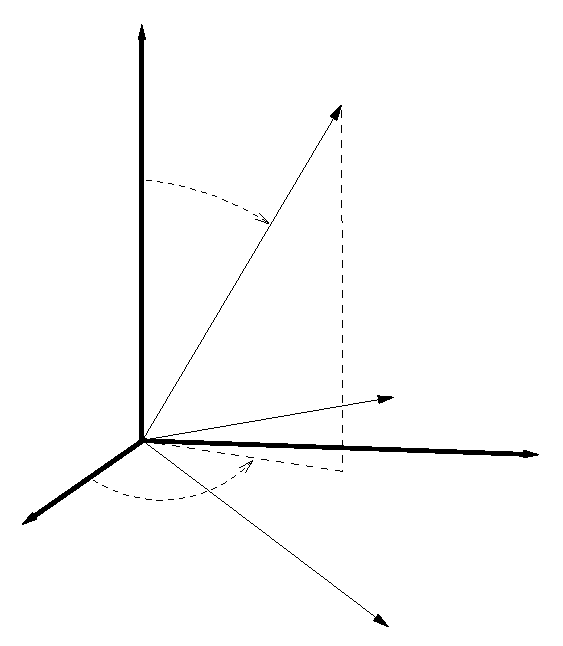
\includegraphics[width=2.5in,clip]{CoordRot}}
\put(0,27){$x$}
\put(175,51){$y$}
\put(37,209){$z$}
\put(128,3){$\acute{x}$}
\put(129,82){$\acute{y}$}
\put(103,181){$\acute{z}$}
\put(40,36){$\bar\alpha$}
\put(63,153){$\bar\beta$}
\end{picture}} 
Each scalar can be expanded in terms of its own set of spin-weighted
spherical harmonics:
\begin{equation}
\Psi_4(\theta,\phi)=\sum_{\ell m}C_{\ell m}\swY{-2}{\ell m}{\theta,\phi}
\qquad\mbox{and}\qquad
\Psi_4(\acute\theta,\acute\phi)=
\sum_{\ell m}\acute{C}_{\ell m}\swY{-2}{\ell m}{\acute\theta,\acute\phi}.
\end{equation}
This gives us
\begin{equation}
\Psi_4(\theta,\phi)=\sum_{\ell m}C_{\ell m}\swY{-2}{\ell m}{\theta,\phi}
=e^{-i(-2)(\Lambda-\phi+\acute\phi)}
\sum_{\ell m}\acute{C}_{\ell m}\swY{-2}{\ell m}{\acute\theta,\acute\phi}.
\end{equation}
Using the orthonormality of the spin-weighted spherical harmonics,
we find
\begin{equation}
C_{\acute\ell\acute{m}}=\oint{\swY[*]{-2}{\acute\ell\acute{m}}{\theta,\phi}
  \left(e^{-i(-2)(\Lambda-\phi+\acute\phi)}
  \sum_{\ell m}\acute{C}_{\ell m}\swY{-2}{\ell m}{\acute\theta,\acute\phi}\right)
  {\rm d}\Omega}
\end{equation}
Allowing for the moment that our coordinates are related by a proper,
homogeneous Lorentz transformation, we can use the inverse of
Eq.~(\ref{eq:LorentzYTrans})
\begin{equation}
\swY{s}{\ell m}{\theta,\phi}=
     K^Le^{-is(\Lambda-\phi+\acute\phi)}\sum_{\acute\ell\acute{m}}
         \mathcal{R}^{-1(s,L)}_{\ell m\acute\ell\acute{m}}
                 \swY{s}{\acute\ell\acute{m}}{\acute\theta,\acute\phi} 
\end{equation}
and transform the area element using Eq.~(\ref{eq:LorentzMetricTrans}) to
get
\begin{eqnarray}
C_{\acute\ell\acute{m}}&=&\oint{
  \left(K^Le^{-i(-2)(\Lambda-\phi+\acute\phi)}\sum_{\hat\ell\hat{m}}
         \mathcal{R}^{-1(s,L)}_{\acute\ell\acute{m}\hat\ell\hat{m}}
                 \swY{-2}{\hat\ell\hat{m}}{\acute\theta,\acute\phi}
\right)^*
  \left(e^{-i(-2)(\Lambda-\phi+\acute\phi)}
  \sum_{\ell m}\acute{C}_{\ell m}\swY{-2}{\ell m}{\acute\theta,\acute\phi}\right)
  K^2{\rm d}\acute\Omega} \\ \mbox{} \label{eq:LorentzCoefTrans}
&=& \sum_{\hat\ell\hat{m}}{\sum_{\ell m}{
 \left(\mathcal{R}^{-1(s,L)}_{\acute\ell\acute{m}\hat\ell\hat{m}}\right)^*
 \acute{C}_{\ell m}
 \oint{K^{L+2}\swY[*]{-2}{\hat\ell\hat{m}}{\acute\theta,\acute\phi}
   \swY{-2}{\ell m}{\acute\theta,\acute\phi}{\rm d}\acute\Omega}}}.
\end{eqnarray}
It is clear that the ``conformal'' factor $K$ spoils the
orthonormality condition in the case of full proper, homogeneous
Lorentz transformations.  However, in the restricted case of
rotations, we have $K=1$.  We also have 
\begin{equation}
  \mathcal{R}^{-1(s,L)}_{\acute\ell\acute{m}\ell m} = 
  D^{\ell*}_{\acute{m}m}(\bar\alpha,\bar\beta,\bar\gamma)\delta_{\acute\ell,\ell},
\end{equation}
allowing us to simplify Eq.~(\ref{eq:LorentzCoefTrans}), after
relabeling indices, to
\begin{equation}
  C_{\ell{m}} = \sum_{\acute{m}}{
    \acute{C}_{\ell\acute{m}}
    D^\ell_{m\acute{m}}(\bar\alpha,\bar\beta,\bar\gamma)}.
\end{equation}

In particular, if our $\acute{C}_{\ell m}$ are from the mode decomposition
of Kerr given in Eq.~(\ref{eq:SphericalKerrModes}), we find that
\begin{equation}\label{eq:SphericalRotatedKerrModes}
\begin{aligned}
 C_{\ell{m}}(t) & = \sum_{\acute\ell\acute{m}n}
 D^{\acute\ell}_{m\acute{m}}(\bar\alpha,\bar\beta,0) \Big\{ 
   A_{\acute\ell\acute{m}n}\YSH{\ell\acute\ell\acute{m}}{c_{\acute\ell\acute{m}n}}
    e^{-i\omega_{\acute\ell\acute{m}n}t+i\phi_{\acute\ell\acute{m}n}}e^{-t/\tau_{\acute\ell\acute{m}n}} \\
& {} \hspace{0.6in}
  + (-1)^{\ell+\ell^\prime} A^\prime_{\acute\ell\acute{m}n}
    \YSH[*]{\ell\acute\ell(-\acute{m})}{c_{\acute\ell(-\acute{m})n}}
    e^{i\omega_{\acute\ell(-\acute{m})n}t-i\phi^\prime_{\acute\ell\acute{m}n}}e^{-t/\tau_{\acute\ell(-\acute{m})n}} \Big\}.
\end{aligned}
\end{equation}
With the Wigner rotation matrices $D^\ell_{mn}(\phi,\theta,\gamma)$
defined as
\begin{equation}
  D^\ell_{m\acute{m}}(\bar\alpha,\bar\beta,\bar\gamma) \equiv 
       e^{-im\bar\alpha} d^\ell_{m\acute{m}}(\bar\beta) e^{-i\acute{m}\bar\gamma},
\end{equation}
it is clear that the $\phi$ coordinate rotation by angle $\bar\alpha$
can be absorbed into the definitions of the
$\phi_{\acute\ell\acute{m}n}$ and $\phi^\prime_{\acute\ell\acute{m}n}$
phase shifts.  So, in the context of trying to fit against data to
find the orientation of the black hole spin axis, it is not possible
to determine the $\phi$ rotation.

Alternatively, if we know the rotation angles of the ``Kerr''
coordinate systems relative to the ``code'' coordinate system, then
we can construct the expansion coefficients $\acute{C}_{\ell{m}}$ via
\begin{equation}
  \acute{C}_{\ell{m}} = \sum_{\acute{m}}{C_{\ell\acute{m}}
                      D^{\ell{*}}_{\acute{m}m}(\bar\alpha,\bar\beta,\bar\gamma)}.
\end{equation}


\newpage
\noindent{\large\bf Appendix: Spectral Method for Spin-Weighted
  Spheroidal Harmonics}
\vspace{0.25in}

We can expand the spin-weighted spheroidal functions in terms of the
spin-weighted spherical functions,
\begin{equation}
  \swS{s}{\ell{m}}{x}{c} = \sum_{\ell^\prime=\ell_{\mbox{\tiny min}}}^\infty
      C_{\ell^\prime\ell{m}}(c)\swS{s}{\ell^\prime{m}}{x}{0},
\end{equation}
where $\ell_{\mbox{min}}\equiv\max(|m|,|s|)$.  Using this expansion in
the first term in Eq.~(\ref{eqn:swSF_DiffEqn}), we get
\begin{align}
   \partial_x \Big[ (1-x^2)\partial_x [\swS{s}{\ell{m}}{x}{c}]\Big]
   &= \sum_{\ell^\prime=\ell_{\mbox{\tiny min}}}^\infty
      C_{\ell^\prime\ell{m}}(c)
      \partial_x \Big[ (1-x^2)\partial_x [\swS{s}{\ell^\prime{m}}{x}{0}]\Big] \\
   &= -\sum_{\ell^\prime=\ell_{\mbox{\tiny min}}}^\infty C_{\ell^\prime\ell{m}}(c)
      \left[s + \ell^\prime(\ell^\prime+1)-s(s+1)-\frac{(m+sx)^2}{1-x^2}\right]
      \swS{s}{\ell^\prime{m}}{x}{0} \\
   &= -\sum_{\ell^\prime=\ell_{\mbox{\tiny min}}}^\infty C_{\ell^\prime\ell{m}}(c)
      \left[\ell^\prime(\ell^\prime+1)\right]
      \swS{s}{\ell^\prime{m}}{x}{0} +
      \left[s^2+\frac{(m+sx)^2}{1-x^2}\right]
      \swS{s}{\ell{m}}{x}{c} \\
   &= -\left[(cx)^2 - 2csx + s+\scA{s}{\ell{m}}{c}-\frac{(m+sx)^2}{1-x^2}\right]
      \swS{s}{\ell{m}}{x}{c}.
\end{align}
The last two lines then give
\begin{equation}
  \left[(cx)^2 - 2csx + s(s+1) +\scA{s}{\ell{m}}{c}\right]
  \swS{s}{\ell{m}}{x}{c} =
  \sum_{\ell^\prime=\ell_{\mbox{\tiny min}}}^\infty C_{\ell^\prime\ell{m}}(c)
  \left[\ell^\prime(\ell^\prime+1)\right]
  \swS{s}{\ell^\prime{m}}{x}{0}
\end{equation}
which we can rewrite as
\begin{equation}
   \sum_{\ell^\prime=\ell_{\mbox{\tiny min}}}^\infty C_{\ell^\prime\ell{m}}(c)
   \left[\ell^\prime(\ell^\prime+1) -s(s+1) - (cx)^2 
     + 2csx -\scA{s}{\ell{m}}{c} \right]
   \swS{s}{\ell^\prime{m}}{x}{0} = 0.
\end{equation}
Eliminating the $x$ and $x^2$ dependence using Eqs~(\ref{eqn:swS:xrecur}) and (\ref{eqn:swS:x2recur}), and relabeling the $\ell^\prime$ indices so that all of the spin-weighted spherical functions $\swS{s}{\ell{m}}{x}{0}$ are of the same order, we get
\begin{align}
- \sum_{\ell^\prime=\ell_{\mbox{\tiny min}}+2}^\infty c^2 C_{(\ell^\prime-2)\ell{m}}(c)
   \mathcal{A}_{s(\ell^\prime-2)m}\swS{s}{\ell^\prime{m}}{x}{0} &
\nonumber \\
-  \sum_{\ell^\prime=\ell_{\mbox{\tiny min}}+1}^\infty C_{(\ell^\prime-1)\ell{m}}(c)
   \left[c^2\mathcal{D}_{s(\ell^\prime-1)m} 
     - 2cs\mathcal{F}_{s(\ell^\prime-1)m}\right]
   \swS{s}{\ell^\prime{m}}{x}{0} &
\nonumber \\
+  \sum_{\ell^\prime=\ell_{\mbox{\tiny min}}}^\infty C_{\ell^\prime\ell{m}}(c)
   \left[[\ell^\prime(\ell^\prime+1) -s(s+1) 
       - c^2 \mathcal{B}_{s\ell^\prime{m}} + 2cs\mathcal{H}_{s\ell^\prime{m}}
       \right]\swS{s}{\ell^\prime{m}}{x}{0} &
\nonumber \\
-  \sum_{\ell^\prime=\ell_{\mbox{\tiny min}}-1}^\infty C_{(\ell^\prime+1)\ell{m}}(c)
   \left[c^2\mathcal{E}_{s(\ell^\prime+1)m} 
     - 2cs\mathcal{G}_{s(\ell^\prime+1)m}\right]
   \swS{s}{\ell^\prime{m}}{x}{0} &
\nonumber \\
- \sum_{\ell^\prime=\ell_{\mbox{\tiny min}}-2}^\infty c^2 C_{(\ell^\prime+2)\ell{m}}(c)
   \mathcal{C}_{s(\ell^\prime+2)m}\swS{s}{\ell^\prime{m}}{x}{0} &
\nonumber \\
=  \sum_{\ell^\prime=\ell_{\mbox{\tiny min}}}^\infty C_{\ell^\prime\ell{m}}(c)&
   \scA{s}{\ell{m}}{c}\swS{s}{\ell^\prime{m}}{x}{0}.
\end{align}

We demand that $\mathcal{F}_{s(\ell_{\mbox{\tiny min}}-1){m}}=0$,
which implies that $\mathcal{A}_{s(\ell_{\mbox{\tiny min}}-1){m}} =
\mathcal{A}_{s(\ell_{\mbox{\tiny min}}-2){m}} =
\mathcal{D}_{s(\ell_{\mbox{\tiny min}}-1){m}}=0$.  This, together with the
fact that $\swS{s}{(\ell_{\mbox{\tiny min}}-1){m}}{x}{0} =
\swS{s}{(\ell_{\mbox{\tiny min}}-2){m}}{x}{0} = 0$, allows us to combine the
terms under one sum, yielding
\begin{align}\label{eqn:eigenvalue_eqn:inf}
\sum_{\ell^\prime=\ell_{\mbox{\tiny min}}}^\infty\Big\{
& - c^2 \mathcal{A}_{s(\ell^\prime-2)m} C_{(\ell^\prime-2)\ell{m}}(c)
-  \left[c^2\mathcal{D}_{s(\ell^\prime-1)m} 
            - 2cs\mathcal{F}_{s(\ell^\prime-1)m}\right] C_{(\ell^\prime-1)\ell{m}}(c)
\nonumber \\
&\mbox{} + \left[[\ell^\prime(\ell^\prime+1) -s(s+1) 
       - c^2 \mathcal{B}_{s\ell^\prime{m}} + 2cs\mathcal{H}_{s\ell^\prime{m}}
       \right] C_{\ell^\prime\ell{m}}(c)
\nonumber  \\
&\mbox{} -  \left[c^2\mathcal{E}_{s(\ell^\prime+1)m} 
            - 2cs\mathcal{G}_{s(\ell^\prime+1)m}\right] C_{(\ell^\prime+1)\ell{m}}(c) 
- c^2 \mathcal{C}_{s(\ell^\prime+2)m} 
       C_{(\ell^\prime+2)\ell{m}}(c)\Big\}\swS{s}{\ell^\prime{m}}{x}{0}
\nonumber \\
& =  \sum_{\ell^\prime=\ell_{\mbox{\tiny min}}}^\infty 
   \scA{s}{\ell{m}}{c} C_{\ell^\prime\ell{m}}(c) \swS{s}{\ell^\prime{m}}{x}{0}.
\end{align}
We find, then, the 5-term recurrence relation
\begin{align}
- c^2 \mathcal{A}_{s(\ell^\prime-2)m} C_{(\ell^\prime-2)\ell{m}}(c)
-  \left[c^2\mathcal{D}_{s(\ell^\prime-1)m} 
            - 2cs\mathcal{F}_{s(\ell^\prime-1)m}\right] C_{(\ell^\prime-1)\ell{m}}(c)&
\nonumber \\
\mbox{} + \left[[\ell^\prime(\ell^\prime+1) -s(s+1) 
       - c^2 \mathcal{B}_{s\ell^\prime{m}} + 2cs\mathcal{H}_{s\ell^\prime{m}}
       \right] C_{\ell^\prime\ell{m}}(c)&
\nonumber  \\
\mbox{} -  \left[c^2\mathcal{E}_{s(\ell^\prime+1)m} 
            - 2cs\mathcal{G}_{s(\ell^\prime+1)m}\right] C_{(\ell^\prime+1)\ell{m}}(c) 
- c^2 \mathcal{C}_{s(\ell^\prime+2)m} 
       C_{(\ell^\prime+2)\ell{m}}(c)
& = \scA{s}{\ell{m}}{c} C_{\ell^\prime\ell{m}}(c).
\end{align}

If we truncate the series at $\ell_{\mbox{\tiny max}}$ then we have a
finite-dimensional spectral approximation to the eigenvalue problem
for the spin-weighted spheroidal harmonics.  With 
$N=\ell_{\mbox{\tiny max}} - \ell_{\mbox{\tiny min}} + 1$, then for
given values of $s$ and $m$, we have an $N\times{N}$ pente-diagonal
matrix $\mathbb{M}$ whose elements are given by
\begin{equation}
  M_{\ell\ell^\prime} = \left\{\begin{array}{lcl}
  \mbox{if\ }\ell^\prime=\ell-2 &:& -c^2 \mathcal{A}_{s\ell^\prime{m}}, \\
  \mbox{if\ }\ell^\prime=\ell-1 &:& -c^2 \mathcal{D}_{s\ell^\prime{m}} 
                                   + 2cs \mathcal{F}_{s\ell^\prime{m}} ,\\
  \mbox{if\ }\ell^\prime=\ell &:& \ell^\prime(\ell^\prime+1)-s(s+1)
                                   - c^2 \mathcal{B}_{s\ell^\prime{m}} 
                                   + 2cs \mathcal{H}_{s\ell^\prime{m}}, \\
  \mbox{if\ }\ell^\prime=\ell+1 &:& -c^2 \mathcal{E}_{s\ell^\prime{m}} 
                                   + 2cs \mathcal{G}_{s\ell^\prime{m}}, \\
  \mbox{if\ }\ell^\prime=\ell+2 &:& -c^2 \mathcal{C}_{s\ell^\prime{m}}, \\
  \mbox{otherwise} &:& 0.
  \end{array}\right.
\end{equation}
The finite dimensional version of Eq.~(\ref{eqn:eigenvalue_eqn:inf}) is 
then simply the eigenvalue equation
\begin{equation}\label{eqn::eigenvalue_eqn:fin}
  \mathbb{M}\cdot\vec{C}_{\ell{m}}(c) = \scA{s}{\ell{m}}{c}\vec{C}_{\ell{m}}(c).
\end{equation}
For given $s$, $m$, and $c$, the matrix $\mathbb{M}$ is constructed
and its $N$ eigenvalues are the $\scA{s}{\ell{m}}{c}$, where $\ell\in
\{\ell_{\mbox{\tiny min}},...,\ell_{\mbox{\tiny max}}\}$, and the
elements of the corresponding eigenvector $\vec{C}_{\ell{m}}(c)$ are the
expansion coefficients $C_{\ell^\prime\ell{m}}(c)$.

Because of the exponential convergence of spectral expansions, for 
$\ell \ge \ell_{\mbox{\tiny min}}$ but $\ell \ll \ell_{\mbox{\tiny max}}$, 
we expect $\scA{s}{\ell{m}}{c}$ and $\vec{C}_{\ell{m}}(c)$ to have
extremely high accuracy.  The largest value of $\ell$ for which we
can expect an accurate eigenvalue and eigenvector can be determined
by looking at the resulting values of the expansion coefficients 
$C_{\ell^\prime\ell{m}}(c)$.  For given $\ell$ and $m$, only coefficients
where $\ell^\prime$ is reasonably close to $\ell$ will have significant
coefficients.  As long as the coefficients $C_{\ell^\prime\ell{m}}(c)$ are
not significant for $\ell^\prime \ge \ell_{\mbox{\tiny max}}$, then 
the solution will be highly accurate.

\newpage
\noindent{\large\bf Appendix: Teukolsky Equation -- Series Solution
of the Radial Equation}
\vspace{0.25in}

The Teukolsky Equation is written as
\begin{equation}
\begin{aligned}
\left[\frac{(r^2+a^2)^2}{\Delta} - a^2\sin^2\theta\right]
   \frac{\partial^2\psi}{\partial{t}^2}
+ \frac{4Mar}{\Delta}\frac{\partial^2\psi}{\partial{t}\partial\phi}
+ \left[\frac{a^2}{\Delta} - \frac1{\sin^2\theta}\right]
   \frac{\partial^2\psi}{\partial\phi^2} &\\
- \Delta^{-s}\frac{\partial}{\partial{r}}\left(
    \Delta^{s+1}\frac{\partial\psi}{\partial{r}}\right)
-  \frac1{\sin\theta}\frac{\partial}{\partial\theta}\left(
   \sin\theta\frac{\partial\psi}{\partial\theta}\right)
- 2s\left[\frac{a(r-M)}{\Delta} + \frac{i\cos\theta}{\sin^2\theta}\right]
     \frac{\partial\psi}{\partial\phi} &\\
- 2s\left[\frac{M(r^2-a^2)}{\Delta} - r - ia\cos\theta\right]
     \frac{\partial\psi}{\partial{t}}
+ (s^2\cot^2\theta - s)\psi
&= 4\pi\Sigma T,
\end{aligned}
\end{equation}
where\\
\parbox{3.75in}{
\begin{align}
  \Delta &\equiv r^2 + a^2 - 2Mr \nonumber \\
         &= (r-r_+)(r-r_\minus)
\end{align}
}
\parbox{3.75in}{
\begin{align}
  \Sigma &\equiv r^2 + a^2\cos^2\theta; \\
    r_\pm &\equiv M \pm \sqrt{M^2 - a^2}
\end{align}
}

With
\begin{equation}
  \psi(t,r,\theta,\phi) = e^{-i\omega{t}} e^{im\phi}S(\theta)R(r),
\end{equation}
the equation separates.  The angular equation is given by
Eq.~(\ref{eqn:swSF_DiffEqn}) with $S(\theta) =
\swS{s}{\ell{m}}{\cos\theta}{a\omega}$, and the radial equation
is given by
\begin{equation}\label{eqn:radialR:Diff_Eqn}
\Delta^{-s}\frac{d}{dr}\left[\Delta^{s+1}\frac{dR(r)}{dr}\right]
+ \left[\frac{K^2 -2is(r-M)K}{\Delta} + 4is\omega{r} - \lambda\right]R(r)=0,
\end{equation}
where
\begin{align}
  K &\equiv (r^2+a^2)\omega - am, \\
  \lambda &\equiv \scA{s}{\ell{m}}{a\omega} + a^2\omega^2 - 2am\omega.
\end{align}

In order to explore the behavior of solutions near the horizon, $r_+$
and near infinity, it is useful to rewrite the differential equation in
terms of the tortoise coordinate $r^*$ defined by
\begin{equation}\label{eqn:tortoise_coord:DiffEqn}
  \frac{dr^*}{dr} \equiv \frac{r^2+a^2}{\Delta}.
\end{equation}
We find
\begin{equation}
\frac{d^2Y(r^*)}{d{r^*}^2} +\left\{\frac1{(r^2+a^2)^2}\left[
    K^2 -2is(r-M)K + \Delta(4is\omega{r} - \lambda)\right]
    - G^2 - \frac{dG}{dr^*}\right\}Y(r^*) = 0,
\end{equation}
where we assume $r=r(r^*)$ and
\begin{align}\label{eqn:radialtortoise:DiffEqn}
  Y(r^*) &\equiv \Delta^{s/2}(r^2+a^2)^{1/2}R(r), \\
  G &\equiv \frac{s(r-M)}{r^2+a^2} + \frac{r\Delta}{(r^2+a^2)^2}.
\end{align}
In the asymptotic limit $r\to\infty$ ($r^*\to\infty$),
Eq.~(\ref{eqn:radialtortoise:DiffEqn}) becomes
\begin{equation}
\frac{d^2Y(r^*)}{d{r^*}^2} + \left(\omega^2 
     + 2\frac{is\omega}{r}\right)Y(r^*) \approx 0,
\end{equation}
which has the two solutions (to the same order)
\begin{equation}
   Y(r^*) \sim r^{\pm{s}}e^{\mp{i}\omega{r^*}}.
\end{equation}
In terms of the original radial function we find
\begin{equation}
  \lim_{r\to\infty}R(r) \sim \left\{\begin{array}{lcl}
      \frac{e^{-i\omega{r^*}}}{r} &:& \mbox{ingoing wave}, \\ \\
      \frac{e^{i\omega{r^*}}}{r^{2s+1}} &:& \mbox{outgoing wave}. \\
   \end{array}\right.
\end{equation}
In the asymptotic limit $r\to r_+$ ($r^*\to-\infty$),
Eq.~(\ref{eqn:radialtortoise:DiffEqn}) becomes
\begin{equation}
\frac{d^2Y(r^*)}{d{r^*}^2} + \left(k 
    - is\frac{(r_+-M)}{2Mr_+}\right)^2Y(r^*) \approx 0,
\end{equation}
where $k\equiv\omega-m\omega_+$ and $\omega_+\equiv a/(2Mr_+)$,
which has the two solutions (to the same order)
\begin{equation}\label{eqn:rplusYlimit}
   Y(r^*) \sim e^{\pm{i}k{r^*}}\left[e^{\frac{(r_+-M)}{Mr_+}r^*}\right]^{\pm{s}/2}.
\end{equation}
In order to determine the asymptotic limit of the term in brackets, we
need to integrate Eq.~(\ref{eqn:tortoise_coord:DiffEqn}) for the
Tortoise coordinates.  The result is
\begin{equation}\label{eqn:Tortose_coord}
  r^* = r + \frac{2M}{r_+-r_\minus}\left[
    r_+\ln\left(\frac{r-r_+}{M}\right) 
    - r_\minus\ln\left(\frac{r-r_\minus}{M}\right)\right].
\end{equation}
To consider the asymptotic limit we let $r=r_++\epsilon$ giving us
\begin{align}
   r^*(\epsilon) &= r_+ + \epsilon + \frac{2M}{r_+-r_\minus}\left[
    r_+\ln\left(\frac{\epsilon}{M}\right) 
    - r_\minus\ln\left(\frac{\epsilon +r_+-r_\minus}{M}\right)\right] \nonumber\\ 
   &= r_+ + \epsilon + \frac{2M}{r_+-r_\minus}\left[
    r_+\ln\left(\frac{\epsilon}{M}\right) 
    - r_\minus\ln\left(1+\frac{\epsilon}{r_+-r_\minus}\right)
   + r_\minus\ln\left(\frac{M}{r_+-r_\minus}\right)\right].
\end{align}
So, the term in brackets in Eq.~(\ref{eqn:rplusYlimit}) becomes
\begin{equation}
  \frac{(r_+-M)}{Mr_+}r^*(\epsilon) =
     \frac{(r_+-M)}{Mr_+}\left[r_+ + \mathcal{O}(\epsilon)\right]
     + 2\frac{(r_+-M)}{r_+-r_\minus}\ln\left(\frac\epsilon{M}\right).
\end{equation}
But $2\frac{(r_+-M)}{r_+-r_\minus}=1$, so
\begin{align}
  e^{\frac{(r_+-M)}{Mr_+}r^*(\epsilon)} &\propto \epsilon + \mathcal{O}(\epsilon^2), \\
       &\propto (r-r_+)(r-r_\minus) + \mathcal{O}(\epsilon^2), \\
       &\propto \Delta + \mathcal{O}(\epsilon^2).
\end{align}
This give us
\begin{equation}
   Y(r^*) \sim \Delta^{\pm{s}/2}e^{\pm{i}k{r^*}},
\end{equation}
or in terms of the original radial function
\begin{equation}
  \lim_{r^*\to-\infty}R(r^*) \sim \left\{\begin{array}{lcl}
      e^{ik{r^*}} &:& \mbox{ingoing wave (out of BH)}, \\ \\
     \Delta^{-s}e^{-ik{r^*}} &:& \mbox{outgoing wave (into BH)}. \\
   \end{array}\right.
\end{equation}
The latter solution, representing waves flowing into the black hole is the physically relevant condition.

Returning to the standard radial coordinate $r$ via
Eq.~(\ref{eqn:Tortose_coord}) gives us the behavior near $\infty$ as
\begin{equation}
  R(r) \sim r^{-1-2s+2i\omega{M}}e^{i\omega{r}}, 
\end{equation}
and near the horizon, $r=r_+$ as
\begin{equation}
  R(r) \sim (r - r_+)^{-s-i\sigma_+}, 
\end{equation}
where $\sigma_\pm\equiv\frac{2\omega{M}r_\pm - ma}{r_+-r_\minus}$, and we
have used $e^{-ik{r^*}} \propto (r-r_+)^{-i\sigma_+}$.

We factor out these asymptotic behaviors by defining a new radial 
function $\bar{R}(r)$ via
\begin{equation}
  R(r) \equiv e^{i\omega{r}} (r-r_\minus)^{-1-s+2i\omega{M}+i\sigma_+} 
        (r - r_+)^{-s-i\sigma_+} \bar{R}(r),
\end{equation}
where we choose $(r-r_\minus)$ in the large $r$ behavior to avoid
introducing singular points near $r=r_+$.
Finally, if we choose dimensionless variables as
\begin{align}
  \bar{r} &\equiv \frac{r}{M}, \\
  \bar{r}_\pm &\equiv \frac{r_\pm}{M}, \\
  \bar\omega &\equiv M\omega, \\
  \bar{a} &\equiv \frac{a}{M},
\end{align}
then our original radial equation, (\ref{eqn:radialR:Diff_Eqn}), can 
be written as
\begin{equation}\label{eqn:radialRbar:Diff_Eqn}
  \Delta^2\frac{d^2\bar{R}(\bar{r})}{d\bar{r}^2}
  + \Delta[b_0 + b_1(\bar{r}-\bar{r}_+) + b_2\Delta]
            \frac{d\bar{R}(\bar{r})}{d\bar{r}}
  + [b_3\Delta + b_4(\bar{r}-\bar{r}_+)]\bar{R}(\bar{r}) = 0,
\end{equation}
where
\begin{align}
  b_0 &\equiv (1-s-2i\sigma_+)(\bar{r}_+-\bar{r}_\minus), \\
  b_1 &\equiv -2(s-2i\bar\omega), \\
  b_2 &\equiv 2i\bar\omega, \\
  b_3 &\equiv (4\bar{r}_+-\bar{a}^2)\bar\omega^2
              + 2[(\bar{r}_+-\bar{r}_\minus)\sigma_+ + i\bar{r}_+ 
                  - 2i(1+s)]\bar\omega - \scA{s}{\ell{m}}{\bar{a}\bar\omega}, \\
  b_4 &\equiv -(\bar{r}_+-\bar{r}_\minus)(1-4i\bar\omega)(1+s-2i\sigma_+),
\end{align}
and we note that Eq.~(\ref{eqn:radialRbar:Diff_Eqn}) has no singular
points at $r=r_+$.

A series expansion can by found for $\bar{R}(\bar{r})$ by choosing
\begin{equation}
  \bar{R}(\bar{r}) = \sum_{n=0}^\infty{a_n\left(
       \frac{\bar{r}-\bar{r}_+}{\bar{r}-\bar{r}_\minus}\right)^n}.
\end{equation}
It is convenient to use a new coordinate $\xi$ which varies over the
range $[0,1]$ and is defined by
\begin{equation}
  \xi \equiv \frac{\bar{r}-\bar{r}_+}{\bar{r}-\bar{r}_\minus}.
\end{equation}
In terms of $\xi$, Eq.~(\ref{eqn:radialRbar:Diff_Eqn}) becomes
\begin{equation}\label{eqn:Rbar_xi:Diff_Eqn}
  \xi(1-\xi)^2\frac{d^2\bar{R}(\xi)}{d\xi^2}
  + [C_0(1-\xi)^2 - C_1\xi(1-\xi) + C_2\xi]
            \frac{d\bar{R}(\xi)}{d\xi}
  + [C_3(\xi-1) + C_4]\bar{R}(\xi) = 0,
\end{equation}
where
\begin{align}
  C_0 &\equiv 1-s-2i\sigma_+, \\
  C_1 &\equiv 2(1+s-2i\bar\omega), \\
  C_2 &\equiv 2i(\bar{r}_+-\bar{r}_\minus)\bar\omega, \\
  C_3 &\equiv (1-4i\bar\omega)(1+s-2i\sigma_+), \\
  C_4 &\equiv (4\bar{r}_+-\bar{a}^2)\bar\omega^2
              + 2[(\bar{r}_+-\bar{r}_\minus)\sigma_+ + i\bar{r}_+ 
                  - 2i(1+s)]\bar\omega - \scA{s}{\ell{m}}{\bar{a}\bar\omega}.
\end{align}
Inserting the series expansion into Eq.~(\ref{eqn:Rbar_xi:Diff_Eqn}), we get
\begin{equation}
\begin{aligned}
  \sum_{n=0}^\infty{a_n\{n(n-1) + n[C_0+C_1] + C_3\}}\xi^{n+1} & \\
  \sum_{n=0}^\infty{a_n\{-2n(n-1) + n[-2C_0-C_1+C_2] + [-C_3+C_4]\}}\xi^n & \\
  \sum_{n=0}^\infty{a_n\{n(n-1) + nC_0\}}\xi^{n-1} &=0.
\end{aligned}
\end{equation}
Relabeling the sums we get
\begin{equation}
\begin{aligned}
  \sum_{n=1}^\infty{a_{n-1}\{(n-1)(n-2) + (n-1)[C_0+C_1] + C_3\}}\xi^n & \\
  \sum_{n=0}^\infty{a_n\{-2n(n-1) + n[-2C_0-C_1+C_2] + [-C_3+C_4]\}}\xi^n & \\
  \sum_{n=-1}^\infty{a_{n+1}(n+1)(n+C_0)}\xi^n &=0.
\end{aligned}
\end{equation}
We can rewrite this with a single sum by starting the sum at
$n=1$.  The result is
\begin{equation}\label{eqn:radialPS:sum}
\begin{aligned}
  a_0D_3 + a_1D_0 +
  \sum_{n=1}^\infty\Bigl\{& a_{n+1}\{(n^2 + (1+D_0)n + D_0\} \\
    & \mbox{} + a_n\{-2n^2 + (2+D_1)n + D_3\} \\
    & \mbox{} + a_{n-1}\{n^2 + (-3+D_2)n + D_4 - D_2 + 2)\}\Bigr\}\xi^n =0,
\end{aligned}
\end{equation}
where
\begin{align}
  D_0 &\equiv C_0, \\
  D_1 &\equiv -2C_0-C_1+C_2, \\
  D_2 &\equiv C_0+C_1, \\
  D_3 &\equiv -C_3+C_4, \\
  D_4 &\equiv C_3.
\end{align}
Finally, since Eq.~(\ref{eqn:radialPS:sum}) must be true for all values
of $\xi$, we find
\begin{align}
  a_0\beta_0 + a_1\alpha_0 &= 0, \\
  a_{n+1}\alpha_n + a_n\beta_n + a_{n-1}\gamma_n &=0, \\
  \alpha_n &\equiv n^2 + (D_0+1)n + D_0, \\
  \beta_n &\equiv -2n^2 + (D_1+2)n + D_3, \\
  \gamma_n &\equiv n^2 + (D_2-3)n +D_4 - D_2 +2.
\end{align}

\newpage
\noindent{\large\bf Teukolsky Equation -- Solution
in terms of the confluent Heun Equation}
\vspace{0.25in}

The radial equation given in Eq.~(\ref{eqn:radialR:Diff_Eqn}) can be
written in terms of the confluent Huen equation.  A useful form of it
is the so-called {\em non-symmetrical canonical form} :
\begin{equation}
\frac{d^2H(z)}{dz^2} 
+ \left(4p + \frac\gamma{z}+\frac\delta{z-1}\right)\frac{dH(z)}{dz}
+ \frac{4\alpha pz -\sigma}{z(z-1)}H(z)=0.
\end{equation}
This differential equation has regular singular points at $z=0$ and
$z=1$, and an irregular singular point at $z=\infty$.  In order to
reduce Eq.~(\ref{eqn:radialR:Diff_Eqn}) to this form, we first make
the following transformation:
\begin{equation}
R(r) = (r-r_+)^\xi(r-r_\minus)^\eta e^{\zeta r}H(r).
\end{equation}
Eq.~(\ref{eqn:radialR:Diff_Eqn}) then takes the form
\begin{eqnarray}
&&\frac{d^2H(r)}{dr^2}
+\left(2\zeta +\frac{1+s+2\xi}{r-r_+}+\frac{1+s+2\eta}{r-r_\minus}\right)
\frac{dH(r)}{dr} \\
&&\mbox{}
+\frac{
\begin{array}{l}
\left[4M\omega^2 + 2\zeta(1+\xi+\eta) + 2s(\zeta+i\omega)\right]r
-a^2\omega^2 - \scA{s}{\ell{m}}{a\omega} \\
\mbox{\hspace{0.5in}} + 2M\left(2M\omega^2 - (1+s)\zeta - is\omega\right) 
- 2\zeta(r_\minus\xi + r_+\eta) + (\xi+\eta) (1+2s+\xi+\eta)
\end{array}
}{(r-r_+)(r-r_\minus)}H(r)=0, \nonumber
\end{eqnarray}
where the parameters $\zeta$, $\xi$, and $\eta$ must be fixed to be
\begin{equation}\label{eq:Teukolsky_Heun_parameters}
  \zeta=\pm i\omega\equiv\zeta_\pm,\qquad
  \xi=\frac{-s\pm(s + 2i\sigma_+)}2\equiv\xi_\pm,\qquad
  \eta=\frac{-s\pm(s - 2i\sigma_\minus)}2\equiv\eta_\pm,
\end{equation}
so that there are 8 possible ways of achieving this form, and we recall that
\begin{equation}
 \sigma_\pm\equiv\frac{2\omega{M}r_\pm - ma}{r_+-r_\minus}
\end{equation}
If we define $\bar\zeta=\pm i\bar\omega$, then we have the dimensionless form
\begin{eqnarray}
&&\frac{d^2H(\bar{r})}{d\bar{r}^2}
+\left(2\bar\zeta +\frac{1+s+2\xi}{\bar{r}-\bar{r}_+}
+\frac{1+s+2\eta}{\bar{r}-\bar{r}_\minus}\right)
\frac{dH(\bar{r})}{d\bar{r}} \\
&&\mbox{}
+\frac{
\begin{array}{l}
\left[4\bar\omega^2 + 2\bar\zeta(1+\xi+\eta) 
+ 2s(\bar\zeta+i\bar\omega)\right]\bar{r}
-\bar{a}^2\bar\omega^2 - \scA{s}{\ell{m}}{\bar{a}\bar\omega} \\
\mbox{\hspace{0.5in}} + 2\left(2\bar\omega^2-(1+s)\bar\zeta-is\bar\omega\right) 
- 2\bar\zeta(\bar{r}_\minus\xi + \bar{r}_+\eta) + (\xi+\eta) (1+2s+\xi+\eta)
\end{array}
}{(\bar{r}-\bar{r}_+)(\bar{r}-\bar{r}_\minus)}H(\bar{r})=0, \nonumber
\end{eqnarray}

There are several choices for transforming the radial coordinate
$\bar{r}$.  We will use
\begin{equation}
z \equiv \frac{\bar{r}-\bar{r}_\minus}{\bar{r}_+-\bar{r}_\minus}.
\end{equation}
We find:
\begin{eqnarray}
  p &=& (\bar{r}_+-\bar{r}_\minus)\frac{\bar\zeta}2 \\
  \gamma &=& 1+s+2\eta \\
  \delta &=& 1+s+2\xi \\
  \alpha &=& 1+s+\xi+\eta - 2\bar\zeta + s\frac{i\bar\omega}{\bar\zeta} \\
  \sigma &=& \scA{s}{\ell{m}}{\bar{a}\bar\omega} + \bar{a}^2\bar\omega^2 
   - 2\left(2\bar\omega^2-(1+s)\bar\zeta-is\bar\omega\right) 
   + 2\bar\zeta(\bar{r}_\minus\xi + \bar{r}_+\eta) - (\xi+\eta) (1+2s+\xi+\eta)
   -2\bar\zeta\alpha\bar{r}_\minus \nonumber\\
   &=& \scA{s}{\ell{m}}{\bar{a}\bar\omega} + \bar{a}^2\bar\omega^2 
   - 8\bar\omega^2 + p(2\alpha+\gamma-\delta)
   + \left(1+s-\frac{\gamma+\delta}2\right)\left(s+\frac{\gamma+\delta}2\right).
\end{eqnarray}

For the regular singular point at $z=0$ ($r=r_\minus$), the
characteristic exponents are $\{0,1-\gamma\}$ so the solutions behave
like
{\em (special behavior if $\gamma$ is an integer)}
\begin{equation}
  \lim_{z\to0}H(z)\sim1 \quad\mbox{or}\quad z^{1-\gamma}.
\end{equation}
For the regular singular point at $z=1$ ($r=r_+$), the characteristic
exponents are $\{0,1-\delta\}$ so the solutions behave like
{\em (special behavior if $\delta$ is an integer)}
\begin{equation}
  \lim_{z\to1}H(z)\sim1 \quad\mbox{or}\quad (z-1)^{1-\delta}.
\end{equation}
For the irregular singular point at $z=\infty$, solutions behave like
{\em (fails iff $p=0$)}
\begin{equation}
  \lim_{z\to\infty}H(z)\sim z^{-\alpha} \quad\mbox{or}\quad 
  e^{-4pz}z^{\alpha-\gamma-\delta}.
\end{equation}
Now, with $R(z)\sim z^\eta(z-1)^\xi e^{(\bar{r}_+-\bar{r}_\minus)\bar\zeta z}H(z)$, we
find
\begin{eqnarray}
  \lim_{z\to0}R(z)&\sim& z^\eta \quad\mbox{or}\quad z^{-s-\eta}, \\
  \lim_{z\to1}R(z)&\sim& (z-1)^\xi \quad\mbox{or}\quad (z-1)^{-s-\xi},\\
  \lim_{z\to\infty}R(z)&\sim& 
z^{-1-s(1+\frac{i\bar\omega}{\bar\zeta})+2\bar\zeta}e^{(\bar{r}_+-\bar{r}_\minus)\bar\zeta z} 
\quad\mbox{or}\quad 
z^{-1-s(1-\frac{i\bar\omega}{\bar\zeta})-2\bar\zeta}e^{-(\bar{r}_+-\bar{r}_\minus)\bar\zeta z}.
\end{eqnarray}
It is easy to see that the behavior at $z=0$ ($r=r_\minus$) depends
only on $\eta$ and that each of the two values of $\eta$ yield the
same pair of local solutions.  The same is true for the two values of
$\xi$ at $z=1$ ($r=r_+$), and for the two values of $\zeta$ at
$z=\infty$.  So any of the 8 possible combinations of the three pairs
of parameters yields the same set of local solutions:
\begin{eqnarray}
  \lim_{z\to0}R(z)&\sim& z^{-s+i\sigma_\minus} \quad\mbox{or}\quad z^{-i\sigma_\minus}, \\
  \lim_{z\to1}R(z)&\sim& (z-1)^{-s-i\sigma_+} \quad\mbox{or}\quad (z-1)^{i\sigma_+},\\
  \lim_{z\to\infty}R(z)&\sim& 
z^{-1-2s+2i\bar\omega}e^{i(\bar{r}_+-\bar{r}_\minus)\bar\omega z} 
\quad\mbox{or}\quad 
z^{-1-2i\bar\omega}e^{-i(\bar{r}_+-\bar{r}_\minus)\bar\omega z}.
\end{eqnarray}
Physical solutions representing radiation that is entering the black-hole
horizon ($z=1$) and is outgoing at infinity are given by
\begin{equation}\label{eq:Phys_R_BCs}
  \lim_{z\to1}R(z)\sim (z-1)^{-s-i\sigma_+} \quad\mbox{and}\quad
  \lim_{z\to\infty}R(z)\sim 
  z^{-1-2s+2i\bar\omega}e^{i(\bar{r}_+-\bar{r}_\minus)\bar\omega z},
\end{equation}
and require $s\le0$.

Two local solutions are defined by
\begin{equation}\label{eq:local_a_sol}
 Hc^{(a)}(p,\alpha,\gamma,\delta,\sigma;0)=1 \quad\mbox{and}\quad
 Hc^{(a)}(p,\alpha,\gamma,\delta,\sigma;z) = \sum_{k=0}^\infty{c^{(a)}_kz^k}
\end{equation}
and
\begin{equation}\label{eq:local_r_sol}
 \lim_{z\to\infty}z^\alpha Hc^{(r)}(p,\alpha,\gamma,\delta,\sigma;z)=1
 \quad\mbox{and}\quad
 Hc^{(r)}(p,\alpha,\gamma,\delta,\sigma;z) = \sum_{k=0}^\infty{c^{(r)}_kz^{-\alpha-k}}.
\end{equation}
{\em Note, there are assumptions about $p$ in the limit for
  $Hc^{(r)}$.}  The coefficients $c^{(a)}_k$ and $c^{(r)}_k$ are
defined by 3-term recurrence relations
\begin{eqnarray}
  f^{(a)}_kc^{(a)}_{k+1}+ g^{(a)}_kc^{(a)}_k+ h^{(a)}_kc^{(a)}_{k-1} &=& 0 
  \qquad c^{(a)}_{-1}=0 \qquad c^{(a)}_0=1 \\
  g^{(a)}_k &=& k(k-4p+\gamma+\delta-1)-\sigma \\
  f^{(a)}_k &=& -(k+1)(k+\gamma) \\
  h^{(a)}_k &=& 4p(k+\alpha-1)
\end{eqnarray}
and
\begin{eqnarray}
  f^{(r)}_kc^{(r)}_{k+1}+ g^{(r)}_kc^{(r)}_k+ h^{(r)}_kc^{(r)}_{k-1} &=& 0 
  \qquad c^{(r)}_{-1}=0 \qquad c^{(r)}_0=1 \\
  g^{(r)}_k &=& (k+\alpha)(k+4p+\alpha-\gamma-\delta+1)-\sigma \\
  f^{(r)}_k &=& -4p(k+1) \\
  h^{(r)}_k &=& -(k+\alpha-1)(k+\alpha-\gamma)
\end{eqnarray}

The physical solution at $z=1$ corresponds to either of the local solutions
\begin{eqnarray}\label{eq:local_sol_z1a}
  Hc^{(a)}(-p,\alpha,\delta,\gamma,\sigma-4p\alpha;1-z) &\mbox{with}&
  \xi=\xi_\minus, \\\label{eq:local_sol_z1b}
  (z-1)^{1-\delta}Hc^{(a)}(-p,\alpha+1-\delta,2-\delta,\gamma,\sigma-(1-\delta)\gamma-4p(\alpha+1-\delta);1-z) &\mbox{with}&
  \xi=\xi_+.
\end{eqnarray}
The physical solution at $z=\infty$ corresponds to either of the local solutions
\begin{eqnarray}\label{eq:local_sol_zinfa}
  Hc^{(r)}(p,\alpha,\gamma,\delta,\sigma;z) &\mbox{with}&
  \bar\zeta=\bar\zeta_+, \\\label{eq:local_sol_zinfb}
  e^{-4pz}Hc^{(r)}(-p,-\alpha+\gamma+\delta,\gamma,\delta,\sigma-4p\gamma;z) &\mbox{with}&
  \bar\zeta=\bar\zeta_\minus.
\end{eqnarray}
The two solutions at $z=0$ correspond to either of the two local solutions
\begin{eqnarray}\label{eq:local_sol_z0a}
  Hc^{(a)}(p,\alpha,\gamma,\delta,\sigma;z) &\mbox{with}&
  \eta=\eta_\pm, \\\label{eq:local_sol_z0b}
  z^{1-\gamma}Hc^{(a)}(p,\alpha+1-\gamma,2-\gamma,\delta,\sigma+(1-\gamma)(4p-\delta);z) &\mbox{with}&
  \eta=\eta_\mp.
\end{eqnarray}

The local solutions $Hc^{(a,r)}(p,-q,\gamma,\delta,\sigma;z)$ can
yield polynomial solutions under certain conditions.  A {\em
  necessary} condition for a polynomial solution to exist is that the
second parameter, $-q$, must be a non-positive integer.  This forces
$h_{q+1}^{(a,r)}=0$.  If $c_{q+1}^{(a,r)}=0$ also holds, then the
infinite series will terminate, yielding a polynomial solution.  This
second condition, referred to as a $\Delta_{q+1}=0$ condition, is
satisfied by the vanishing of the determinant
\begin{equation}\label{eq:Delta_q_cond}
  \left|\begin{array}{ccccc}
  g_0 & f_0 & 0 & \cdots & 0 \\
  h_1 & g_1 & f_1 & \ddots & 0 \\
  0 & h_2 & g_2 & \ddots & 0 \\
  0 & 0 & \ddots & \ddots & \ddots \\
  0 & 0 & \cdots & h_q & g_q
  \end{array}\right|
\end{equation}
and will be discussed further below.

The necessary condition that the second parameter be a non-positive
integer, $-q$, can be satisfied in several ways.  First consider
\begin{equation}\label{eq:PP_boundary_set}
  q= \left\{\begin{array}{cc}
            -\alpha & (\bar\zeta_+,\xi_\minus,\eta_\pm) \\
            -\alpha-1+\delta & (\bar\zeta_+,\xi_+,\eta_\pm) \\
            \alpha-\gamma-\delta & (\bar\zeta_\minus,\xi_\minus,\eta_\pm) \\
            -\alpha-1+\gamma & (\bar\zeta_+,\xi_\minus,\eta_\mp)
  \end{array}\right\} =\left\{\begin{array}{c}
  -1-s+i\frac{2\bar\omega(1+\sqrt{1-\bar{a}^2})-\bar{a}m}{\sqrt{1-\bar{a}^2}} \\
  -1+4i\bar{\omega}
  \end{array}\right. .
\end{equation}
The first column in the first set of brackets corresponds to the four
versions of the second parameter in
Eqs.~(\ref{eq:local_sol_z1a})--(\ref{eq:local_sol_z0b}).  The second
column corresponds to the particular choice for each of the three
parameters given in Eq.~(\ref{eq:Teukolsky_Heun_parameters}).  The
$\zeta$ parameter fixes the two possible boundary conditions at
infinity.  The $\xi$ parameter, the two possible boundary conditions
at the black hole horizon.  And the $\eta$ parameter fixes the two
possible conditions at inner (or Cauchy) horizon.  All four version
for $q$ represent same physical solution, but where $H(z)$ has been
redefined leading to a version of the Heun equation with different
coefficients.

For each version of $q$ in this set, the parameters are chosen to
yield waves that are in-going (into the black-hole) at the horizon and
out-going at infinity [see Eq.~(\ref{eq:Phys_R_BCs})].  These are the
``physical'' boundary conditions that can yield QNMs.  It also assumes
the local solutions behave as in Eqs.~(\ref{eq:local_a_sol})
and~(\ref{eq:local_r_sol}).  The boundary conditions at the horizon
and at infinity are independent of the choice for the $\eta$
parameter, so this set of values for $q$ corresponds to two distinct
solutions distinguished by the choice of the boundary condition at the
inner horizon.  The two equations following the final bracket
correspond to the values of $q$ for these two possible choices for
$\eta$.  The top equation corresponds to the ``upper'' choice for
$\eta$ and the bottom equation to the ``lower'' choice.  Note that for
$q=-\alpha-1+\gamma$, the choices for $\eta$ are reversed.  Since $q$
must be a non-negative integer, we see that these conditions fix the
value of $\bar\omega$.  The upper choice requires
\begin{equation}\label{eq:PP_omega_upper}
  \bar\omega = \frac{\bar{a}m-iN\sqrt{1-\bar{a}^2}}{2(1+\sqrt{1-\bar{a}^2})}
  \quad;\qquad N\ge 1+s,\ N\in\,\rm{Integers}.
\end{equation}
The lower choice requires
\begin{equation}\label{eq:PP_omega_lower}
  \bar\omega = -i\frac{N}4 \quad;\qquad N\ge 1,\ N\in\,\rm{Integers}.
\end{equation}

There are 3 other sets of conditions on the second parameter.  If we
consider the so-called Total-Transmission Mode left (TTM${}_{\rm{L}}$)
case where waves are again out-going at infinity, but the non-physical
boundary condition of waves coming out of the black-hole horizon is
chosen, then we find
\begin{equation}\label{eq:NP_boundary_set}
  q= \left\{\begin{array}{cc}
            -\alpha & (\bar\zeta_+,\xi_+,\eta_\pm) \\
            -\alpha-1+\delta & (\bar\zeta_+,\xi_\minus,\eta_\pm) \\
            \alpha-\gamma-\delta & (\bar\zeta_\minus,\xi_+,\eta_\pm) \\
            -\alpha-1+\gamma & (\bar\zeta_+,\xi_+,\eta_\mp)
  \end{array}\right\} =\left\{\begin{array}{c}
  -1-2s \\
  -1-s-i\frac{2\bar\omega(1-\sqrt{1-\bar{a}^2})-\bar{a}m}{\sqrt{1-\bar{a}^2}}
  \end{array}\right. .
\end{equation}  
In this case, the upper choice does not fix $\bar\omega$, but only requires
$s\le-\frac12$.  The lower choice requires
\begin{equation}
  \bar\omega = \frac{\bar{a}m+iN\sqrt{1-\bar{a}^2}}{2(1-\sqrt{1-\bar{a}^2})}
  \quad;\qquad N\ge 1+s,\ N\in\,\rm{Integers},
\end{equation}
unless $\bar{a}=0$, in which case it is only necessary that $s\le-1$.

The Total-Transmision Mode right (TTM${}_{\rm{R}}$) case represents
a physical boundary condition at the horizon and waves that are
in-coming at infinity.  In this case, we find
\begin{equation}\label{eq:PN_boundary_set}
  q= \left\{\begin{array}{cc}
            -\alpha & (\bar\zeta_\minus,\xi_\minus,\eta_\pm) \\
            -\alpha-1+\delta & (\bar\zeta_\minus,\xi_+,\eta_\pm) \\
            \alpha-\gamma-\delta & (\bar\zeta_+,\xi_\minus,\eta_\pm) \\
            -\alpha-1+\gamma & (\bar\zeta_\minus,\xi_\minus,\eta_\mp)
  \end{array}\right\} =\left\{\begin{array}{c}
  -1+s+i\frac{2\bar\omega(1-\sqrt{1-\bar{a}^2})-\bar{a}m}{\sqrt{1-\bar{a}^2}} \\
  -1+2s
  \end{array}\right. .
\end{equation}  
In this case, the upper choice requires
\begin{equation}
  \bar\omega = \frac{\bar{a}m-iN\sqrt{1-\bar{a}^2}}{2(1-\sqrt{1-\bar{a}^2})}
  \quad;\qquad N\ge 1-s,\ N\in\,\rm{Integers},
\end{equation}
unless $\bar{a}=0$, in which case it is only necessary that
$s\ge1$. The lower choice does not fix $\bar\omega$, but only requires
$s\ge\frac12$.

Finally, we can consider the case of a bound state where waves are
coming out of the horizon and coming in from infinity.  In this case,
we find
\begin{equation}\label{eq:NN_boundary_set}
  q= \left\{\begin{array}{cc}
            -\alpha & (\bar\zeta_\minus,\xi_+,\eta_\pm) \\
            -\alpha-1+\delta & (\bar\zeta_\minus,\xi_\minus,\eta_\pm) \\
            \alpha-\gamma-\delta & (\bar\zeta_+,\xi_+,\eta_\pm) \\
            -\alpha-1+\gamma & (\bar\zeta_\minus,\xi_+,\eta_\mp)
  \end{array}\right\} =\left\{\begin{array}{c}
  -1-4i\bar\omega \\
  -1+s-i\frac{2\bar\omega(1+\sqrt{1-\bar{a}^2})-\bar{a}m}{\sqrt{1-\bar{a}^2}}
  \end{array}\right. .
\end{equation} 
In this case, both choices for $\eta$ fix $\bar\omega$.  The upper
choice gives requires
\begin{equation}
  \bar\omega = i\frac{N}4 \quad;\qquad N\ge 1,\ N\in\,\rm{Integers}.
\end{equation} 
The lower choice requires
\begin{equation}
  \bar\omega = \frac{\bar{a}m+iN\sqrt{1-\bar{a}^2}}{2(1+\sqrt{1-\bar{a}^2})}
  \quad;\qquad N\ge 1-s,\ N\in\,\rm{Integers}.
\end{equation}

Given the necessary conditions to find polynomial solutions in these
four cases, we must now consider the $\Delta_{q+1}$ condition.  This
condition can be viewed as an eigenvalue problem for the fifth
parameter, $\sigma$, in $Hc^{(a,r)}(p,-q,\gamma,\delta,\sigma;z)$. The
eigenvalues of the matrix in Eq.~(\ref{eq:Delta_q_cond}) must be equal
to $\sigma$.  The $q+1$ eigenvalues are labeled
$\sigma_{0q},\sigma_{1q},\ldots,\sigma_{qq}$ and the polynomial
solution associated with $\sigma_{nq}$ is denoted as
\begin{equation}
  Hc_{nq}(p,\gamma,\delta;z).
\end{equation}

The simplest case to consider this that for the ``upper''
TTM${}_{\rm{L}}$ solutions where $q=-1-2s$
[Eq.~(\ref{eq:NP_boundary_set})].  The requirement that $s\le\frac12$
is sensible given that the Teukolsky equation requires $s\le0$ to
represent out-going waves at infinity.  Since the choice for $q$ in
this solution has not fixed $\bar\omega$, the $\Delta_{q+1}$ condition
will fix the allowed values for $\bar\omega$.

For gravitational perturbations, $s=-2$ so $q=3$.  Polynomial
solutions can be found using any of the six local solutions given by
Eqs.~(\ref{eq:local_sol_z1a})--(\ref{eq:local_sol_z0b})), however it
is easiest to use Eqs.~(\ref{eq:local_sol_z0a}).  For the non-spinning
case, $\bar{a}=0$, we find the 4 eigenvalues associated with
Eq.~(\ref{eq:local_sol_z0a}) to be:
\begin{equation}
\sigma_{03}=-1-\sqrt{1-12i\bar\omega},\quad
\sigma_{13}=-1-\sqrt{1+12i\bar\omega},\quad
\sigma_{23}=-1+\sqrt{1-12i\bar\omega},\quad
\sigma_{33}=-1+\sqrt{1+12i\bar\omega}.
\end{equation}
Values for $\bar\omega$ are obtained from the requirement that
$\sigma_{nq}=\sigma$.  In this case, with $\bar{a}=0$, we have
$\sigma=\scA{-2}{\ell{m}}{0}=\ell(\ell+1)-2$.  Since $\sigma>0$, both
$\sigma_{03}$ and $\sigma_{13}$ are not allowed.  For the other
two solutions, we have
\begin{eqnarray}
  \sigma_{23}&\to&\bar\omega=\frac{i}{12}(\ell-1)\ell(\ell+1)(\ell+2), \\
  \sigma_{33}&\to&\bar\omega=-\frac{i}{12}(\ell-1)\ell(\ell+1)(\ell+2).
\end{eqnarray}
Since the imaginary part of $\bar\omega$ is positive for
$\sigma_{23}$ this solution is unstable, so the physical solution is
obtained from $\sigma_{33}$.  The associated solution is
\begin{equation}\label{eq:TTML_a0_H_sol1}
  Hc_{33}(i\bar\omega,-1,-1+4i\bar\omega;z) = z^2-\frac{l(l+1)}3z^3
\end{equation}
which corresponds to the physical solution
\begin{equation}\label{eq:TTML_a0_R_sol1}
  R(z) = z^2(z-1)^{2i\bar\omega}\left(1-\frac{l(l+1)}3z\right)e^{2i\bar\omega z}.
\end{equation}

For the general case with $\bar{a}\ne0$, we can again use the
solutions associated with Eq.~(\ref{eq:local_sol_z0a}).  We must find
the eigenvalues of
\begin{equation}\label{eq:gen_poly_matrix}
  \left[\begin{array}{cccc}
    -\sigma_{n3} & 
    1-2i\bar\omega+i\frac{2\bar\omega-am}{\sqrt{1-\bar{a}^2}} &
    0 & 0 \\
    -12i\bar\omega\sqrt{1-\bar{a}^2} &
    -2 + 4i\bar\omega\left(1-\sqrt{1-\bar{a}^2}\right) - \sigma_{n3} &
    -4i\bar\omega + 2i\frac{2\bar\omega-am}{\sqrt{1-\bar{a}^2}} &
    0 \\
    0 & -8i\bar\omega\sqrt{1-\bar{a}^2} &
    -2 + 8i\bar\omega\left(1-\sqrt{1-\bar{a}^2}\right) - \sigma_{n3} &
    -3 - 6i\bar\omega + 3i\frac{2\bar\omega-am}{\sqrt{1-\bar{a}^2}} \\
    0 & 0 & -4i\bar\omega\sqrt{1-\bar{a}^2} &
    12i\bar\omega\left(1-\sqrt{1-\bar{a}^2}\right) - \sigma_{n3}
  \end{array}\right]
\end{equation}
and then solve the equation
\begin{equation}\label{eq:gen_sigma_val}
  \sigma_{n3}=\sigma = \scA{-2}{\ell{m}}{\bar{a}\bar\omega} 
    + \bar{a}^2\bar\omega^2 + \bar\omega\left(
       6i\left(1-\sqrt{1-\bar{a}^2}\right) - 2\bar{a}m\right)
\end{equation}
for the value of $\bar\omega$.  Equivalently, we can instert the value
of $\sigma$ from Eq.~(\ref{eq:gen_sigma_val}) into the matrix of
Eq.~(\ref{eq:gen_poly_matrix}) and set the determinant equal to zero.
The result is
\begin{equation}\label{eq:Starobinsky_const}
  0=\lambdabar^2(\lambdabar+2)^2 
  + 8\lambdabar\bar{a}\bar\omega\left(
      6(\bar{a}\bar\omega+m) -5\lambdabar(\bar{a}\bar\omega-m)\right)
      + 144\bar\omega^2\left(1+\bar{a}^2(\bar{a}\bar\omega-m)^2\right),
\end{equation}
where
\begin{equation}
  \lambdabar=\lambdabar_\minus\equiv \scA{-2}{\ell{m}}{\bar{a}\bar\omega}
     + \bar{a}^2\bar\omega^2 - 2m\bar{a}\bar\omega,
\end{equation}
and the right-hand-side of Eq.~(\ref{eq:Starobinsky_const}) is just the
magnitude squared of the Starobinsky constant.

The ``lower'' TTM${}_{\rm{L}}$ solution is somewhat more complicated.
With $s=-2$ we see that, in general, only $q=0$ results in
$\rm{Im}(\bar\omega)<0$ so that a solution would be stable.  The
associated matrix is one-dimensional and trivial, with vanishing
eigenvalue.  In this case, since $\bar\omega$ is fixed, we must find
that an eigenvalue equals $\sigma$ in order for a polynomial solution
to exist.  In this case, $\sigma$ is a function of $\bar{a}$, $m$, and
$\scA{-2}{\ell{m}}{\bar{a}\bar\omega}$.  The $\Delta_{q+1}$ condition
is not satisfied and no solution exists for arbitrary $\bar{a}$.  However,
if $\bar{a}=0$, and $s=-2$, we find $q=1$.  The eigenvalue condition
immediately yields
\begin{equation}
\sigma_{01}=1-\sqrt{1+12i\bar\omega},\quad
\sigma_{11}=1+\sqrt{1+12i\bar\omega}.
\end{equation}
With $\sigma_{01}$ not allowed because it is negative, we find
\begin{equation}
   \sigma_{11}\to\bar\omega =-\frac{i}{12}(\ell-1)\ell(\ell+1)(\ell+2).
\end{equation}
The associated solution is
\begin{equation}\label{eq:TTML_a0_H_sol2}
  Hc_{11}(i\bar\omega,3,-1+4i\bar\omega;z) = 1-\frac{l(l+1)}3z
\end{equation}
which corresponds to the physical solution
\begin{equation}\label{eq:TTML_a0_R_sol2}
  R(z) = z^2(z-1)^{2i\bar\omega}\left(1-\frac{l(l+1)}3z\right)e^{2i\bar\omega z}.
\end{equation}

Interestingly, we find that Eqs.~(\ref{eq:TTML_a0_R_sol1})
and~(\ref{eq:TTML_a0_R_sol2}), supposedly differing in the boundary
condition on the inner horizon, are the same.  On closer examination,
we note that both solutions satisfy the ``lower'' boundary condition
on the inner horizon.  This occurs because, in the limit $a=0$,
$\gamma=-1$ and we find that the characteristic exponents
$\{0,1-\gamma\}$ differ by an integer.  Only the series solution
  corresponding to the larger exponent will be in the form of a simple
  polynomial.  The second solution will usually include a logaritmic term,
  and can be found given the first solution by means of the method of 
variation of constants.

When $a\ne0$, $\gamma=-1-i\sigma_\minus$ which will not be an integer.
Therefore a polynomial solution for the ``upper'' boundary condition
at the inner horizon will exist for the TTM${}_{\rm{L}}$ case when
$a\ne0$.  These solutions are the well-known ``algebraically special''
solutions which have been studied in the past.  Interestingly, we see
that the behavior of the solution at the inner horizon as $a\to0$ is
slightly complicated.  For $a>0$, we see that the local behavior is
$\lim_{z\to0}R(z)\sim z^{-i\sigma_\minus}$, while for $a=0$ it seems
we can have a linear combination of two solutions.  The first is a
polynomial solution that behaves like $\lim_{z\to0}R(z)\sim z^2$.  The
second is obtained by the method of variation of constants.  This
solution is non-polynomial, so we must examine its local behavior at
each of the singular points.  For the inner horizon we find
$\lim_{z\to0}R(z)\sim 1$. This local solution does include logarithmic
terms multiplied by powers of $z$, all of which vanish as $z\to0$.
For the event horizon we find $\lim_{z\to1}R(z)\sim
A(z-1)^{2-2i\bar\omega}+B(z-1)^{2-4i\bar\omega}\ln(z-1)$.  This violates
the desired boundary condition at the event horizon, thus the second
solution is not allowed for the TTM${}_{\rm L}$ case.

Now consider the QNM case corresponding to
Eqs.~(\ref{eq:PP_boundary_set}), (\ref{eq:PP_omega_upper}), and
(\ref{eq:PP_omega_lower}).  Focusing again on the case of
gravitational waves with $s=-2$, we see that both choices for the
inner boundary behavior fix the value for $\bar\omega$.  This means we
must find an eigenvalue of the $\Delta_{q+1}$ condition that equals
$\sigma$ in order for a polynomial solution to exist.  The ``upper''
QNM case is similar to the ``lower'' TTM${}_{\rm L}$ case where
$\sigma$ and the eigenvalues are independent functions of $\bar{a}$
and polynomial solutions do not exist in general.  However, if
$\bar{a}=0$, the $\Delta_{q+1}$ condition is satisfied when
$N=\frac13(l-1)l(l+1)(l+2)$ giving polynomial solutions at the same
set of frequencies found for the $TTM{}_{\rm L}$ case.  Of course, the
``lower'' QNM case must yield the same solutions as the ``upper'' case
when $\bar{a}=0$ since characteristic exponents for $z=0$ differ by an
integer.  In addition, the characteristic exponents for $z=1$ also
differ by an integer for $\bar{a}=0$.  This means that the polynomial
solutions we find for $\bar{a}=0$ will always correspond to the same
boundary condition at the event horizon.  As we have seen, this is the
non-physical condition of the solution flowing out of the black hole.

As with the TTM${}_{\rm L}$ case, we can again consider the solutions
generated from our polynomial solutions at $\bar{a}=0$ by the method
of variation of constants.  This allows us to examine the interesting
problem of whether or not QNM solutions exist along the Negative
Imaginary Axis (NIA) at the special frequencies corresponding to the
TTM${}_{\rm L}$ modes.  As we saw when examining the TTM${}_{\rm L}$
case, the second solution behaves like $\lim_{z\to1}R(z)\sim
A(z-1)^{2-2i\bar\omega}+B(z-1)^{2-4i\bar\omega}\ln(z-1)$ at the event
horizon.  The first term is the behavior for solutions that are
flowing into the event horizon, the desired physical condition for
QNMs.  However, the logarithmic term represents a different divergent
behavior that can be dominant when $i\bar\omega$ for $l>2$.  This
logarithmic term, however, turns out to be irrelevant.  If we consider
the behavior of this second solution at infinity, we find
$\lim_{z\to\infty}R(z)\sim z^{-1-2i\bar\omega}e^{-2i\bar\omega z}$
which represents a solution that is incoming from infinity, violating
the QNM boundary condition.  Since we have found both solutions
to the equation at the desired frequencies on the NIA, and since 
neither corresponds to the QNM conditions, we can conclude that
no QNM solutions exist at these frequencies on the NIA.

For the TTM${}_{\rm R}$ case of Eq.~(\ref{eq:PN_boundary_set}), we a
required to consider cases with positive $s$ corresponding to incoming
waves at infinity.  For the case of gravitational waves with $s=2$, we
find that the ``upper'' condition on the inner boundary yields
solutions only when $\bar{a}=0$ and these solutions are unstable with
$\rm{Im}(\bar\omega)>0$.  The ``lower'' condition corresponds to
  $q=3$ and yields one physical solution with
\begin{equation}
  \sigma_{33}=-1+\sqrt{1+12i\bar\omega} \to
  \bar\omega=-\frac{i}{12}(\ell-1)\ell(\ell+1)(\ell+2).
\end{equation}
The associated solution is
\begin{equation}
  Hc_{33}(-i\bar\omega,-1,-1-4i\bar\omega;z)=
  1 + (\ell-1)(\ell+2)z + \frac13(\ell-1)^2(\ell+2)^2z^2\left(
  1 + \frac{\ell(\ell+1)}3 z\right)
\end{equation}
which corresponds to the physical solution
\begin{equation}
R(z)=z^{-2}(z-1)^{-2-2i\bar\omega}\left[
  1 + (\ell-1)(\ell+2)z + \frac13(\ell-1)^2(\ell+2)^2z^2\left(
  1 + \frac{\ell(\ell+1)}3 z\right)\right]e^{-2i\bar\omega}.
\end{equation}
For the general case with $\bar{a}\ne0$, we must find the eigenvalues of
\begin{equation}\label{eq:gen_poly_matrix2}
  \left[\begin{array}{cccc}
    -\sigma_{n3} & 
    1+2i\bar\omega-i\frac{2\bar\omega-am}{\sqrt{1-\bar{a}^2}} &
    0 & 0 \\
    12i\bar\omega\sqrt{1-\bar{a}^2} &
    -2 - 4i\bar\omega\left(1-\sqrt{1-\bar{a}^2}\right) - \sigma_{n3} &
    4i\bar\omega - 2i\frac{2\bar\omega-am}{\sqrt{1-\bar{a}^2}} &
    0 \\
    0 & 8i\bar\omega\sqrt{1-\bar{a}^2} &
    -2 - 8i\bar\omega\left(1-\sqrt{1-\bar{a}^2}\right) - \sigma_{n3} &
    -3 + 6i\bar\omega - 3i\frac{2\bar\omega-am}{\sqrt{1-\bar{a}^2}} \\
    0 & 0 & 4i\bar\omega\sqrt{1-\bar{a}^2} &
    -12i\bar\omega\left(1-\sqrt{1-\bar{a}^2}\right) - \sigma_{n3}
  \end{array}\right]
\end{equation}
and then solve the equation
\begin{equation}\label{eq:gen_sigma_val2}
  \sigma_{n3}=\sigma = \scA{2}{\ell{m}}{\bar{a}\bar\omega} 
    + \bar{a}^2\bar\omega^2 - \bar\omega\left(
       6i\left(1-\sqrt{1-\bar{a}^2}\right) + 2\bar{a}m\right)+4
\end{equation}
for the value of $\bar\omega$.  Equivalently, we can insert the value
of $\sigma$ from Eq.~(\ref{eq:gen_sigma_val}) into the matrix of
Eq.~(\ref{eq:gen_poly_matrix}) and set the determinant equal to zero.
The result is the same as Eq.~(\ref{eq:Starobinsky_const}), except
that
\begin{equation}
  \lambdabar=\lambdabar_+\equiv \scA{2}{\ell{m}}{\bar{a}\bar\omega}
     + \bar{a}^2\bar\omega^2 - 2m\bar{a}\bar\omega+4.
\end{equation}
However, since
$\scA{-s}{\ell{m}}{\bar{a}\bar\omega}=\scA{s}{\ell{m}}{\bar{a}\bar\omega}+2s$,
we find $\lambdabar_+=\lambdabar_\minus$ yielding the known result
that the TTM${}_{\rm L}$ and TTM${}_{\rm R}$ cases share the same
frequency spectrum.

Finally, the case of bound states given by Eq.~(\ref{eq:NN_boundary_set})
yields no stable modes as expected.



\vspace{0.25in}
Non-polynomial solutions can be obtained by first making the transformation
\begin{equation}
  H(z) = z^{-\alpha}\bar{R}(z).
\end{equation}
If we then choose $\zeta=\zeta_+$ and $\xi=\xi_\minus$, then we
guarantee that the characteristic exponents at $z=1$
($\bar{r}=\bar{r}_+$) and at infinity are zero.  (Note that this is
independent of the choice for $\eta$.)  Next, we let
$z\mapsto\frac{z-1}{z}$, so that the regular singular point at
$\bar{r}_\minus$ is now pushed to $z=-\infty$, the regular singular
point at $\bar{r}_+$ is now located at $z=0$, and the irregular
singular point at infinity is now located at $z=1$.  The differential
equation now becomes
\begin{equation}\label{eq:Leaver_radDE_form}
  z(1-z)^2\frac{d^2\hat{R}(z)}{dz^2} 
     + \left[D_0 + D_1z + D_2z^2\right]\frac{d\hat{R}(z)}{dz} 
     + \left[D_3 + D_4z\right]\hat{R}(z) = 0,
\end{equation}
with $\bar{R}(z)=\hat{R}((z-1)/z)$ and
\begin{eqnarray}
  D_0 &=& \delta = 1+s+2\xi, \\
  D_1 &=& 4p-2\alpha+\gamma-\delta-2, \\
  D_2 &=& 2\alpha-\gamma+2, \\
  D_3 &=& \alpha(4p-\delta)-\sigma, \\
  D_4 &=& \alpha(\alpha-\gamma+1).
\end{eqnarray}
Expanding $\hat{R}(z)$ in Eq.~(\ref{eq:Leaver_radDE_form}) in terms of
the Taylor-series $\hat{R}(z)=\sum_{n=0}^\infty{a_nz^n}$, we obtain
the 3-term recurrence relation where the coefficients, $a_n$, satisfy
\begin{align}\label{eq:Leaver_rad_2-term}
  a_0\beta_0 + a_1\alpha_0 &= 0, \\ \label{eq:Leaver_rad_3-term}
  a_{n+1}\alpha_n + a_n\beta_n + a_{n-1}\gamma_n &=0, \\
  \alpha_n &\equiv n^2 + (D_0+1)n + D_0, \\
  \beta_n &\equiv -2n^2 + (D_1+2)n + D_3, \\
  \gamma_n &\equiv n^2 + (D_2-3)n +D_4 - D_2 +2.
\end{align}

If we let $\rho\equiv\lim_{n\to\infty}\frac{a_{n+1}}{a_n}$, then we obtain 
from Eq.~(\ref{eq:Leaver_rad_3-term}) the characteristic equation
\begin{equation}\label{eqn:a_ratio_characteristic}
  \lim_{n\to\infty}\left\{\frac{a_{n+1}}{a_n}+\frac{\beta_n}{\alpha_n}+
  \frac{a_{n-1}}{a_n}\frac{\gamma_n}{\alpha_n}\right\}=\rho-2+\frac1{\rho}=0.
\end{equation}
So, the radius of convergence is one, but unfortunately, this does not
have distinct roots, so we must consider higher order behavior in
$\lim_{n\to\infty}\frac{a_{n+1}}{a_n}$.  We assume
\begin{equation}\label{eqn:a_ratio_expansion}
  \lim_{n\to\infty}\frac{a_{n+1}}{a_n} = 1 + \frac{u_1}{\sqrt{n}}
      + \frac{u_2}{n} + \frac{u_3}{n^{\frac32}} +\cdots.
\end{equation}
If we consider
\begin{equation}
  \left(\lim_{n\to\infty}\frac{ \frac{d}{dn}a_{n+1}}{a_n}\right) \approx
   \lim_{n\to\infty}\left(\frac{a_{n+1}-a_n}{a_n}\right) =
   \frac{u_1}{\sqrt{n}} + \frac{u_2}{n} + \frac{u_3}{n^{\frac32}} +\cdots,
\end{equation}
then
\begin{equation}\label{eq:residual_def}
  \lim_{n\to\infty}\ln(a_n) \approx \int\left(\frac{u_1}{\sqrt{n}} 
    + \frac{u_2}{n} + \frac{u_3}{n^{\frac32}} +\cdots\right)dn.
\end{equation}
The result is
\begin{equation}\label{eq:asymptotic_a}
  \lim_{n\to\infty}a_n \propto 
  \lim_{n\to\infty}n^{u_2}\exp\left[2u_1\sqrt{n}-2\frac{u_3}{\sqrt{n}} 
    +\cdots\right] 
  = \lim_{n\to\infty}n^{u_2} e^{2u_1\sqrt{n}}.
\end{equation}
If we now insert Eq.~(\ref{eqn:a_ratio_expansion}) into the left hand
side of Eq.~(\ref{eqn:a_ratio_characteristic}) and expand in powers of
$1/\sqrt{n}$, then each power of $n$ must vanish independently and we
can solve for the unknowns $u_i$.  We find
\begin{eqnarray}
  u_1 &=& \pm\sqrt{-(D_0+D_1+D_2)} =\pm\sqrt{-4p} \\
    &=& \pm\sqrt{-2(\bar{r}_+-\bar{r}_\minus)\bar\zeta}, \\
  u_2 &=& -\frac14(4D_0+2D_1+7) = -\frac14(8p-4\alpha+2\gamma+2\delta+3) \\
    &=& -(\bar{r}_+-\bar{r}_\minus+2)\bar\zeta 
        + s\frac{i\bar\omega}{\bar\zeta} -3/4, \\
  u_3 &=& \frac1{32u_1}\left[8D_0(4D_0+2D_2+7)+4D_1(8D_0+D_1+12)
                             +40D_2-16(D_3+D_4)+3\right] \\
      &=& \frac1{32u_1}\left[32p(2p-4\alpha+\gamma+3\delta+4) 
                +4(\gamma+\delta)(\gamma+\delta-2) +16\sigma+3\right].
\end{eqnarray}
The asymptotic behavior of $a_n$ is dominated by the exponential term
in Eq.~(\ref{eq:asymptotic_a}), and the two solutions for $u_1$
correspond to the two possible asymptotic behaviors for $a_n$.  The
solution where $\rm{Re}(u_1)<0$ yields the minimal solution and the
other the dominant solution.  With
$\bar\zeta=\bar\zeta_+=i\bar\omega$, so long as
$\rm{Im}(\bar\omega)<0$, $\rm{Re}(\sqrt{-4p})<0$ and $u_1=+\sqrt{-4p}$
is associated with the minimal solution and $u_1=-\sqrt{-4p}$ with a
dominant solution.

Let us define the ratio $r_n\equiv\frac{a_{n+1}}{a_n}$, then
Eq.~(\ref{eq:Leaver_rad_3-term}) can be written as
\begin{equation}
  \frac{a_{n+1}}{a_n} \equiv r_n 
  = \frac{-\gamma_{n+1}}{\beta_{n+1}+ \alpha_{n+1}r_{n+1}}
  \qquad n=0,1,2,\cdots,
\end{equation}
which is a recursive form equivalent to the continued fraction
\begin{equation}\label{eq:Leaver_rad_CF_dom}
r_n 
  = \frac{-\gamma_{n+1}}{\beta_{n+1}-} 
    \frac{\alpha_{n+1}\gamma_{n+2}}{\beta_{n+2}-}
    \frac{\alpha_{n+2}\gamma_{n+3}}{\beta_{n+3}-}\cdots.
\end{equation}
The usefulness of this continued fraction comes from a theorem due to
Pincherle:
 \\ {\em The continued fraction $r_0$ converges if and only
  if the recurrence relation Eq.~(\ref{eq:Leaver_rad_3-term}) possesses
  a minimal solution $a_n=f_n$, with $f_0\ne0$.  In case of
  convergence, moreover, one has $\frac{f_{n+1}}{f_n}=r_n$ with
  $n=0,1,2,\cdots$ provided $f_n\ne0$.}  The physical solution we seek
will be this minimal solution.  Moreover, because the recurrence
terminates, we have the special condition given by
Eq.~(\ref{eq:Leaver_rad_2-term}).  This tells us that
\begin{equation}\label{eq:termination_cond}
  r_0=\frac{f_1}{f_0}=-\frac{\beta_0}{\alpha_0}.
\end{equation}
So, the continued fraction $r_0$ does converge, but not to just any
value.  It must converge to the specific value given by
Eq.~(\ref{eq:termination_cond}), the termination condition for the
recurrence relation, and this will only be possible when $\bar\omega$
takes on certain values (the QNM).  We rewrite
$r_0=-\frac{\beta_0}{\alpha_0}=\frac{-\gamma_{n+1}}{\beta_{n+1}+
  \alpha_{n+1}r_{n+1}}$ as the continued fraction:
\begin{equation}\label{eq:Leaver_Cf_inf}
  0=\beta_0 -\frac{\alpha_0\gamma_1}{\beta_1-}
             \frac{\alpha_1\gamma_2}{\beta_2-}
             \frac{\alpha_2\gamma_3}{\beta_3-}\cdots.
\end{equation}
Now, define the truncated continued fraction $\rm{Cf}(N)$ by
\begin{equation}\label{eq:Leaver_Cf_N}
  \rm{Cf}(N) = \beta_0 -\frac{\alpha_0\gamma_1}{\beta_1-}
             \frac{\alpha_1\gamma_2}{\beta_2-}
             \frac{\alpha_2\gamma_3}{\beta_3-}\cdots
             \frac{\alpha_{N-1}\gamma_N}{\beta_N+\alpha_N r_N}.
\end{equation}
It is also useful to define the $n^{\rm th}$ inversion of this
truncated continued fraction $\rm{Cf}(n;N)$:
\begin{equation}\label{eq:Leaver_Cf_N_inv}
  \rm{Cf}(n;N) = \beta_n-\frac{\alpha_{n-1}\gamma_n}{\beta_{n-1}-}
                         \frac{\alpha_{n-2}\gamma_{n-1}}{\beta_{n-2}-}
                         \cdots\frac{\alpha_0\gamma_1}{\beta_0}
                         -\frac{\alpha_n\gamma_{n+1}}{\beta_{n+1}-}
                          \frac{\alpha_{n+1}\gamma_{n+2}}{\beta_{n+2}-}
                          \cdots\frac{\alpha_{N-1}\gamma_N}{\beta_N+\alpha_N r_N},
\end{equation}
with $\rm{Cf}(0;N)\equiv\rm{Cf}(N)$ and $0\le n<N$.

For fixed $s$, $m$, and $a$, and for a given value of
$\scA{s}{\ell{m}}{\bar{a}\bar\omega}$, we can solve for the
eigenvalues $\bar\omega$ of Eq.~(\ref{eq:Leaver_radDE_form}) by
finding the roots of Eq.~(\ref{eq:Leaver_Cf_inf}).  In practice, the
continued fraction must be truncated by some means.  Using Lentz's
method, $N$ is determined dynamically by demanding that the change in
$\rm{Cf}(n;N)$ caused by adding additional terms is below some
tolerance.  This is a ``top-down'' approach, evaluating the continued
fraction as a ratio of two infinite series.  With this method, the a
value for $r_N$ is never needed.  An alternate method is to choose a
value for $N$, assume $r_N=0$, and evaluate $\rm{Cf}(n;N)$ from the
``bottom-up''.  With this method, one must test various values of $N$
to ensure that the desired tolerance in $\rm{Cf}(n;N)$ has been
reached.  An even better approach, first used in the context of QNM by
Nollert, is to use Eq.~(\ref{eqn:a_ratio_expansion}) with $n\mapsto N$ to
approximate $r_N$.


\vspace*{0.5in}

Another useful form is the so-called {\em symmetrical canonical form}.  If
we let $z\mapsto 1-2z$, then we have regular singular points at $z=\pm1$
and an irregular singular point at $z=-\infty$, and the differential
equation becomes:
\begin{equation}
\frac{d^2H^{(s)}(z)}{dz^2} 
+ \left(-2p + \frac\gamma{z-1}+\frac\delta{z+1}\right)\frac{dH^{(s)}(z)}{dz}
+ \frac{-2\alpha pz -\sigma+2\alpha p}{z^2-1}H^{(s)}(z)=0,
\end{equation}
Where $H^{(s)}(z)\equiv H(\frac{1-z}2)$.
It is more common to replace $\{\gamma,\delta,\alpha,\sigma\}$ with
$\{\mu,\nu,\beta,\lambda\}$ where:
\begin{equation}
 \gamma=\mu+\nu+1,\qquad \delta=\mu-\nu+1,\qquad \alpha=-\beta+\mu+1,\qquad
\sigma = \lambda -2p(\beta-\mu-\nu-1)-\mu(\mu+1).
\end{equation}
Then the equation is written:
\begin{equation}
\frac{d^2H^{(s)}(z)}{dz^2} 
+ \left(-2p + \frac{\mu+\nu+1}{z-1}+\frac{\mu-\nu+1}{z+1}\right)\frac{dH^{(s)}(z)}{dz}
+ \frac{2p(\beta-\mu-1)z -2p\nu+\mu(\mu+1)-\lambda}{z^2-1}H^{(s)}(z)=0,
\end{equation}
and
\begin{eqnarray}
  \mu &=& s+\eta+\xi \\
  \nu &=& \eta-\xi \\
  \beta &=& 2\bar\zeta - s\frac{i\bar\omega}{\bar\zeta} \\
  \lambda &=& \scA{s}{\ell{m}}{\bar{a}\bar\omega} + s(1+s)
    + \bar{a}^2\bar\omega^2 - 8\bar\omega^2.
\end{eqnarray}

The {\em B\^{o}cher symmetrical form}, also called the {\em
  generalized spheroidal equation}, is obtained by the transformation:
\begin{equation}
  H^{(B)}(z)\equiv(z-1)^{\frac{\mu+\nu}2}(z+1)^{\frac{\mu-\nu}2}e^{-pz}H^{(s)}(z),
\end{equation}
and takes the form:
\begin{equation}
\frac{d}{dz}\left((z^2-1)\frac{dH^{(B)}(z)}{dz}\right)
+\left(-p^2(z^2-1)+2p\beta z-\lambda
    -\frac{\mu^2+\nu^2+2\mu\nu z}{z^2-1}\right)H^{(B)}(z)=0.
\end{equation}

Finally, the {\em normal symmetrical form}, or the {\em normal form of
the  generalized spheroidal equation}, is obtained by the transformation:
\begin{equation}
  H^{(B)}(z)\equiv(1-z^2)^{-\frac12}H^{(N)}(z),
\end{equation}
and takes the form:
\begin{equation}
(z^2-1)\frac{d^2H^{(N)}(z)}{dz^2}
+\left(-p^2(z^2-1)+2p\beta z-\lambda
    -\frac{\mu^2+\nu^2-1+2\mu\nu z}{z^2-1}\right)H^{(N)}(z)=0.
\end{equation}

The differential equation for the spin-weighted spheroidal function
$\swS{s}{\ell{m}}{x}{c}$, Eq.~(\ref{eqn:swSF_DiffEqn}), is another 
example of the confluent Heun equation, this time in the B\^{o}cher 
symmetrical form with
\begin{equation}
  p=c \qquad \beta=s \qquad \lambda=\scA{s}{\ell m}{c}+s(s+1)
\end{equation}
and any of the 8 possible combinations of
\begin{equation}
  \mu = \pm m\quad\hbox{and}\quad\nu=\pm s
  \qquad\mbox{or}\qquad \mu = \pm s\quad\hbox{and}\quad\nu=\pm m.
\end{equation}
Unfortunately, the polynomial solutions do are not the regular
solutions we seek and solution methods in terms of $Hc^{a}$ do not at
present seem advantageous.

\end{document}
